\mainmatter
\pagestyle{headings}
\chapter{Research}
\label{ch:research}

\section{Analysis}
The whole data set and data analysis script can be found on the GitHub repository\footnote{https://github.com/MoutPessemier/A-Survey-On-The-Impact-of-Customer-Chatbots-on-E-commerce}.\\
\break
The data has been anonymised in Excel. A new column was created called 'taskCategory'. The tasks performed are categorised in one of the following 4 categories:
\begin{itemize}
	\item FAQ
	\item Personalised question
	\item Complaint
	\item Sales
\end{itemize}
From the 65 entries, 5 had to be thrown away:
\begin{itemize}
	\item 3 because of the used chatbot: they were no telecom chatbots.
	\item 1 entry was a duplicate.
	\item 1 entry responded with one answer only (only yes and only neutral in part 2)
\end{itemize}

\subsection{Environment Variables}
\subsubsection{Age}
The age variable has an overall mean value of 26,28 and a standard deviation of 7,49. If age gets grouped by the different providers, the following is generated. The mean and standard deviation values for each provider respectively are:
\begin{itemize}
	\item Telenet: 26,96 \& 9,73
	\item Proximus: 27,26 \& 6,07
	\item Orange: 22,5 \& 2,12
	\item T-Mobile: 22,44 \& 2,01
	\item KPN: 27,75 \& 3,59
\end{itemize}
Next to the plot, there is a frequency table that shows the different values for age appearing in this survey, ordered from most common to least common.
\begin{figure}[!htb]
	\minipage{0.75\textwidth}
	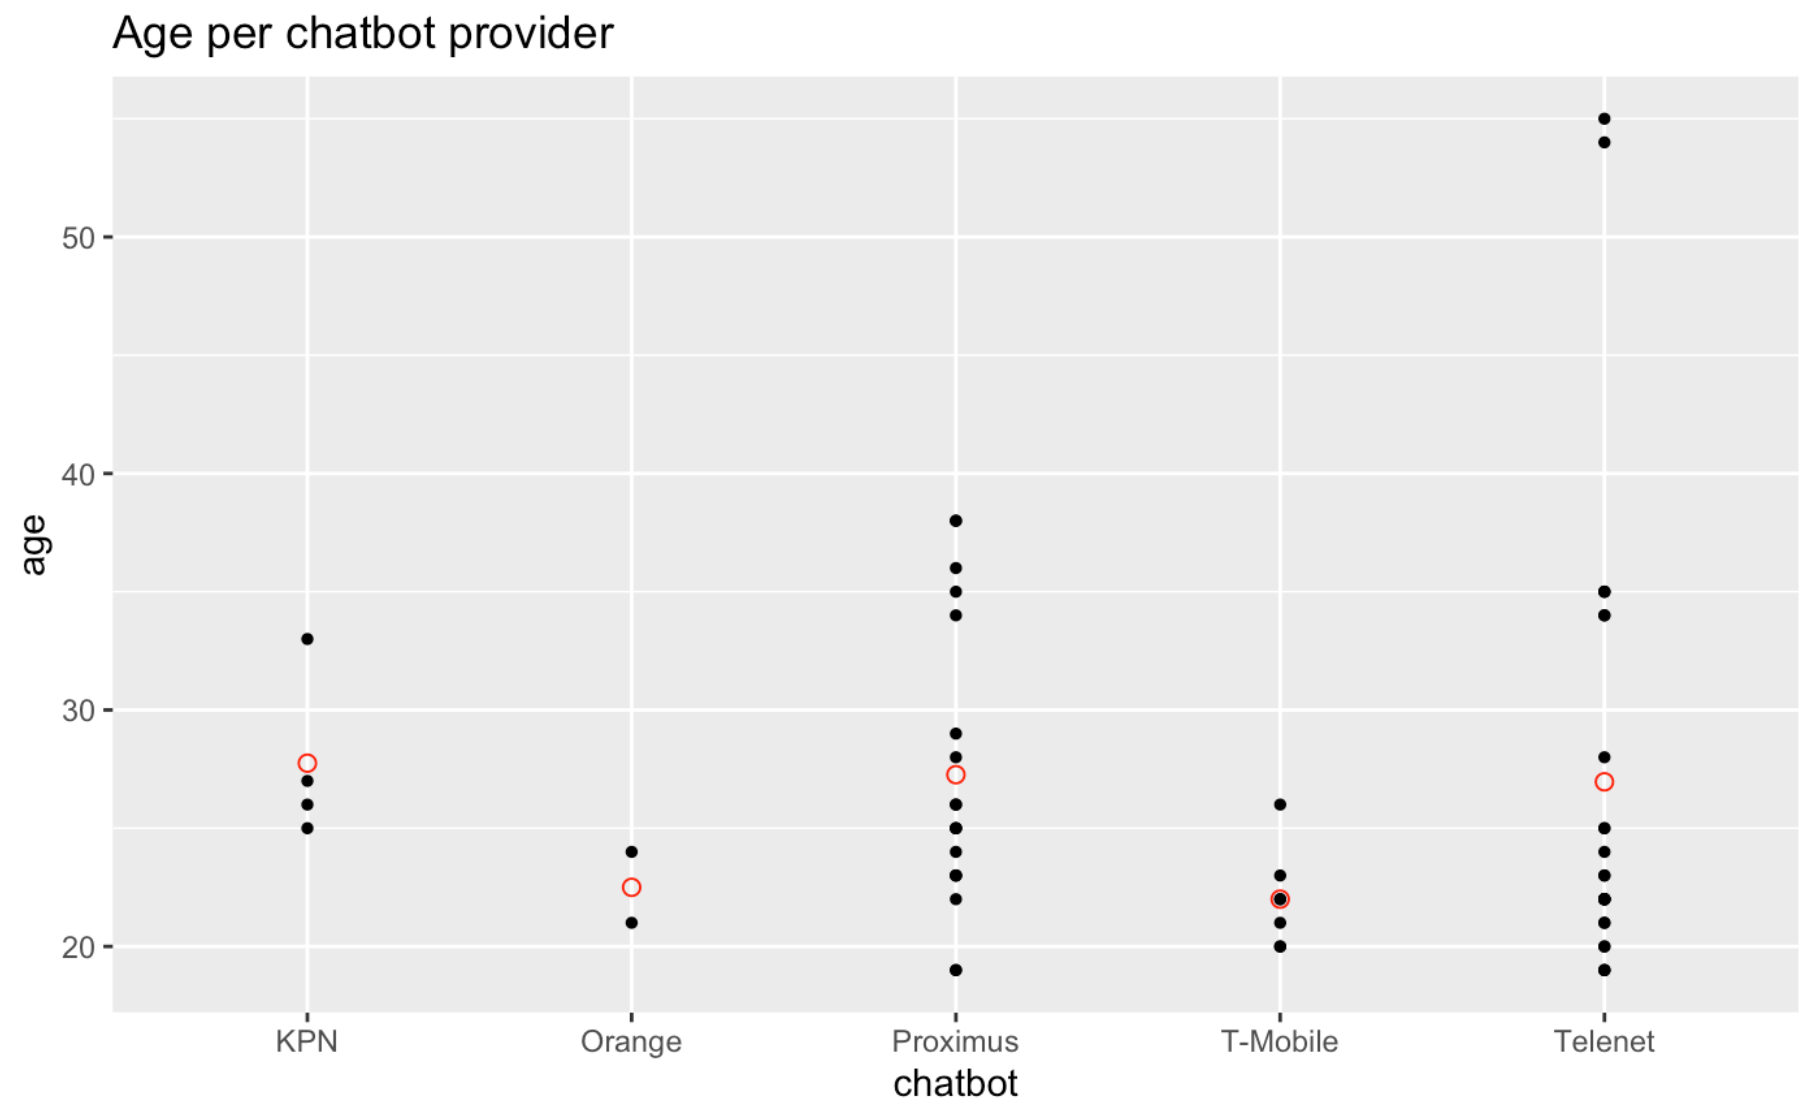
\includegraphics[width=\linewidth]{../LaTeX/Figures/Environments/AgePlot.png}
	\caption{The distribution of the age variable per chatbot provider.}\label{fig:agePlot}
	\endminipage\hfill
	\minipage{0.24\textwidth}
	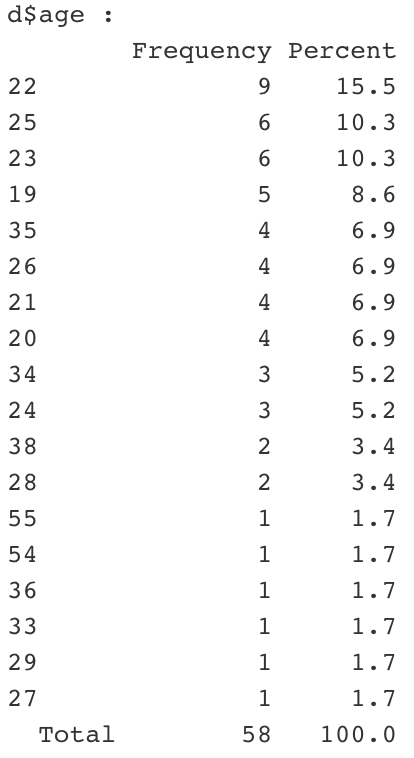
\includegraphics[width=\linewidth]{../LaTeX/Figures/Environments/AgeFreq.png}
	\caption{A frequency table of all the entries' ages.}\label{fig:ageFreq}
	\endminipage\hfill
\end{figure}

\subsubsection{Highest degree}
Looking at the acquired degrees of the respondents, the most common category is a master degree with 19 respondents, followed by an academic bachelor with 17 answers. Third comes high school with 12.
\begin{figure}[!htb]
	\minipage{0.55\textwidth}
	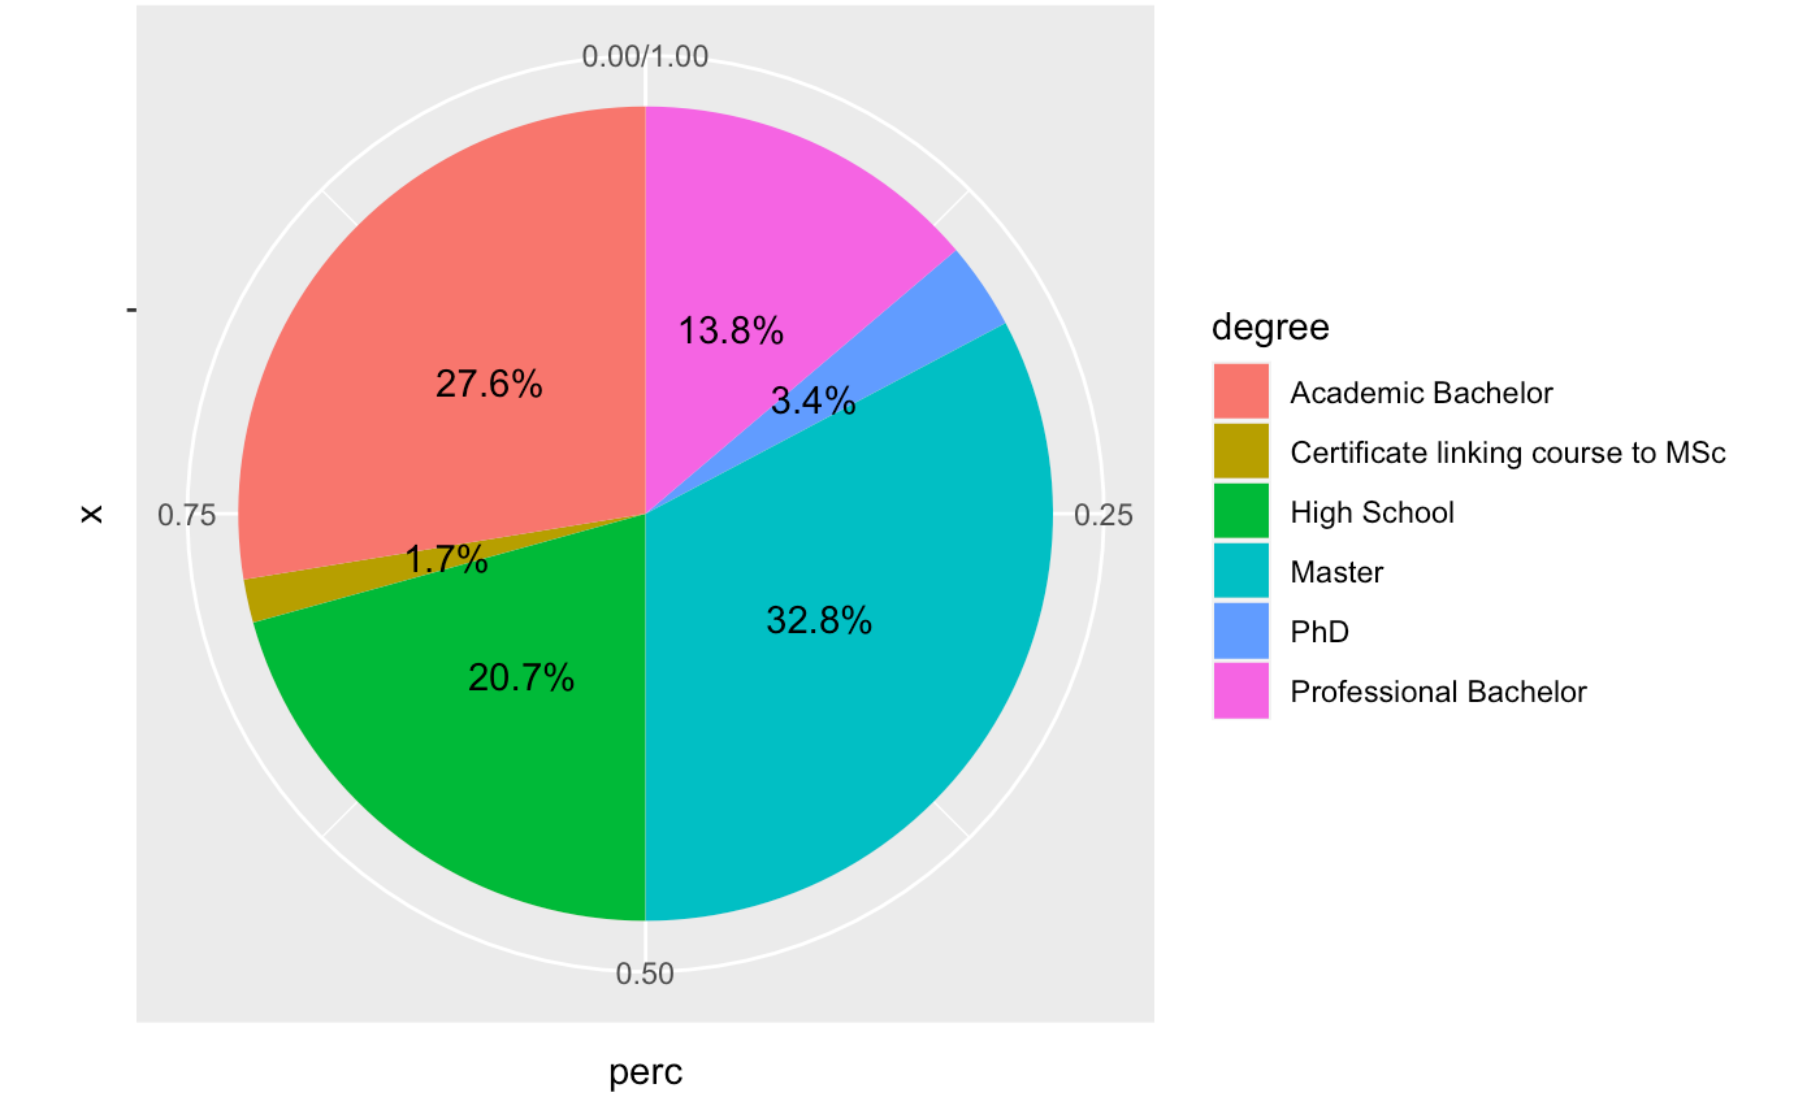
\includegraphics[width=\linewidth]{../LaTeX/Figures/Environments/DegreePlot.png}
	\caption{The distribution of the degree variable.}\label{fig:degreePlot}
	\endminipage\hfill
	\minipage{0.44\textwidth}
	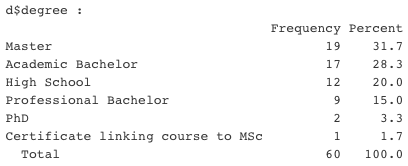
\includegraphics[width=\linewidth]{../LaTeX/Figures/Environments/DegreeFreq.png}
	\caption{A frequency table of all the entries' degrees.}\label{fig:degreeFreq}
	\endminipage\hfill
\end{figure}

\subsubsection{Gender}
There were 34 males who filled in the survey and 25 females. One person identified as non-binary.
\begin{figure}[!htb]
	\minipage{0.69\textwidth}
	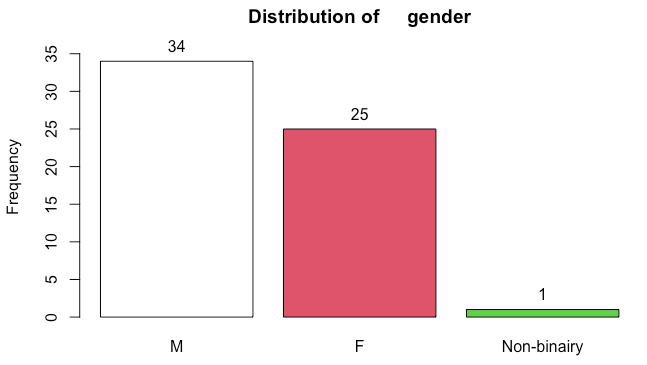
\includegraphics[width=\linewidth]{../LaTeX/Figures/Environments/GenderPlot.png}
	\caption{The distribution of the gender variable.}\label{fig:genderPlot}
	\endminipage\hfill
	\minipage{0.30\textwidth}
	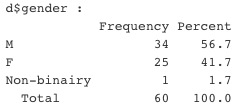
\includegraphics[width=\linewidth]{../LaTeX/Figures/Environments/GenderFreq.png}
	\caption{A frequency table of all the entries' genders.}\label{fig:genderFreq}
	\endminipage\hfill
\end{figure}

\subsubsection{Company of chatbot}
Telenet has the most respondents, followed by Proximus. The other chatbot providers are less represented.
\begin{figure}[!htb]
	\minipage{0.69\textwidth}
	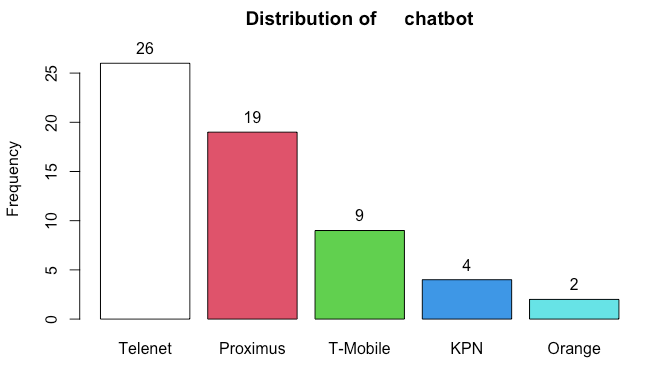
\includegraphics[width=\linewidth]{../LaTeX/Figures/Environments/ChatbotPlot.png}
	\caption{The distribution of the different chatbot providers and the amount of respondents for each provider.}\label{fig:chatbotPlot}
	\endminipage\hfill
	\minipage{0.30\textwidth}
	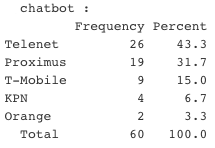
\includegraphics[width=\linewidth]{../LaTeX/Figures/Environments/ChatbotFreq.png}
	\caption{A frequency table of all the entries' used chatbots.}\label{fig:chatbotFreq}
	\endminipage\hfill
\end{figure}

\subsubsection{Used language}
Most users used Dutch as their preferred language of interaction which doesn't come as a surprise since this thesis focuses on the Flemish part of Belgium along with the Netherlands. Afterwards, English was the second most used language and French came last.
\begin{figure}[!htb]
	\minipage{0.69\textwidth}
	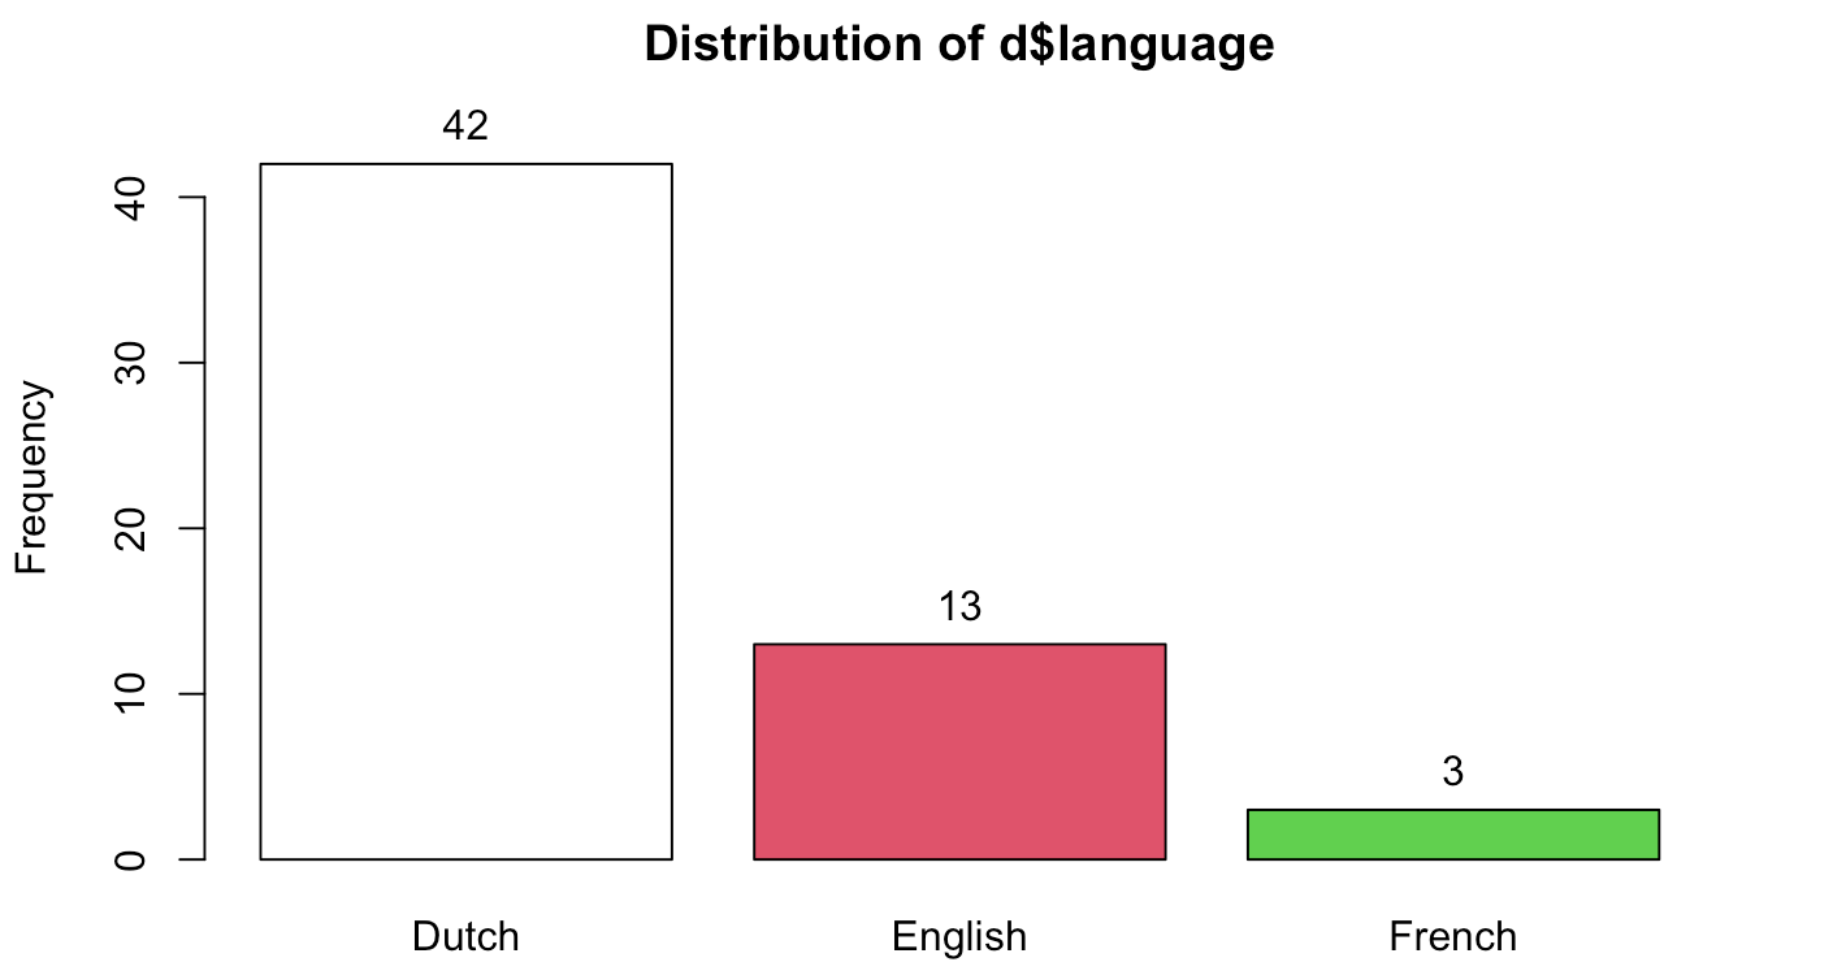
\includegraphics[width=\linewidth]{../LaTeX/Figures/Environments/LanguagePlot.png}
	\caption{The distribution of the language variable.}\label{fig:languagePlot}
	\endminipage\hfill
	\minipage{0.30\textwidth}
	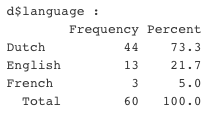
\includegraphics[width=\linewidth]{../LaTeX/Figures/Environments/LanguageFreq.png}
	\caption{A frequency table of all the entries' used languages.}\label{fig:languageFreq}
	\endminipage\hfill
\end{figure}

\subsubsection{Platform}
Most chatbots were used on the website of the provider themselves. Only a small percentage were used in app or via Facebook Messenger.
\begin{figure}[!htb]
	\minipage{0.69\textwidth}
	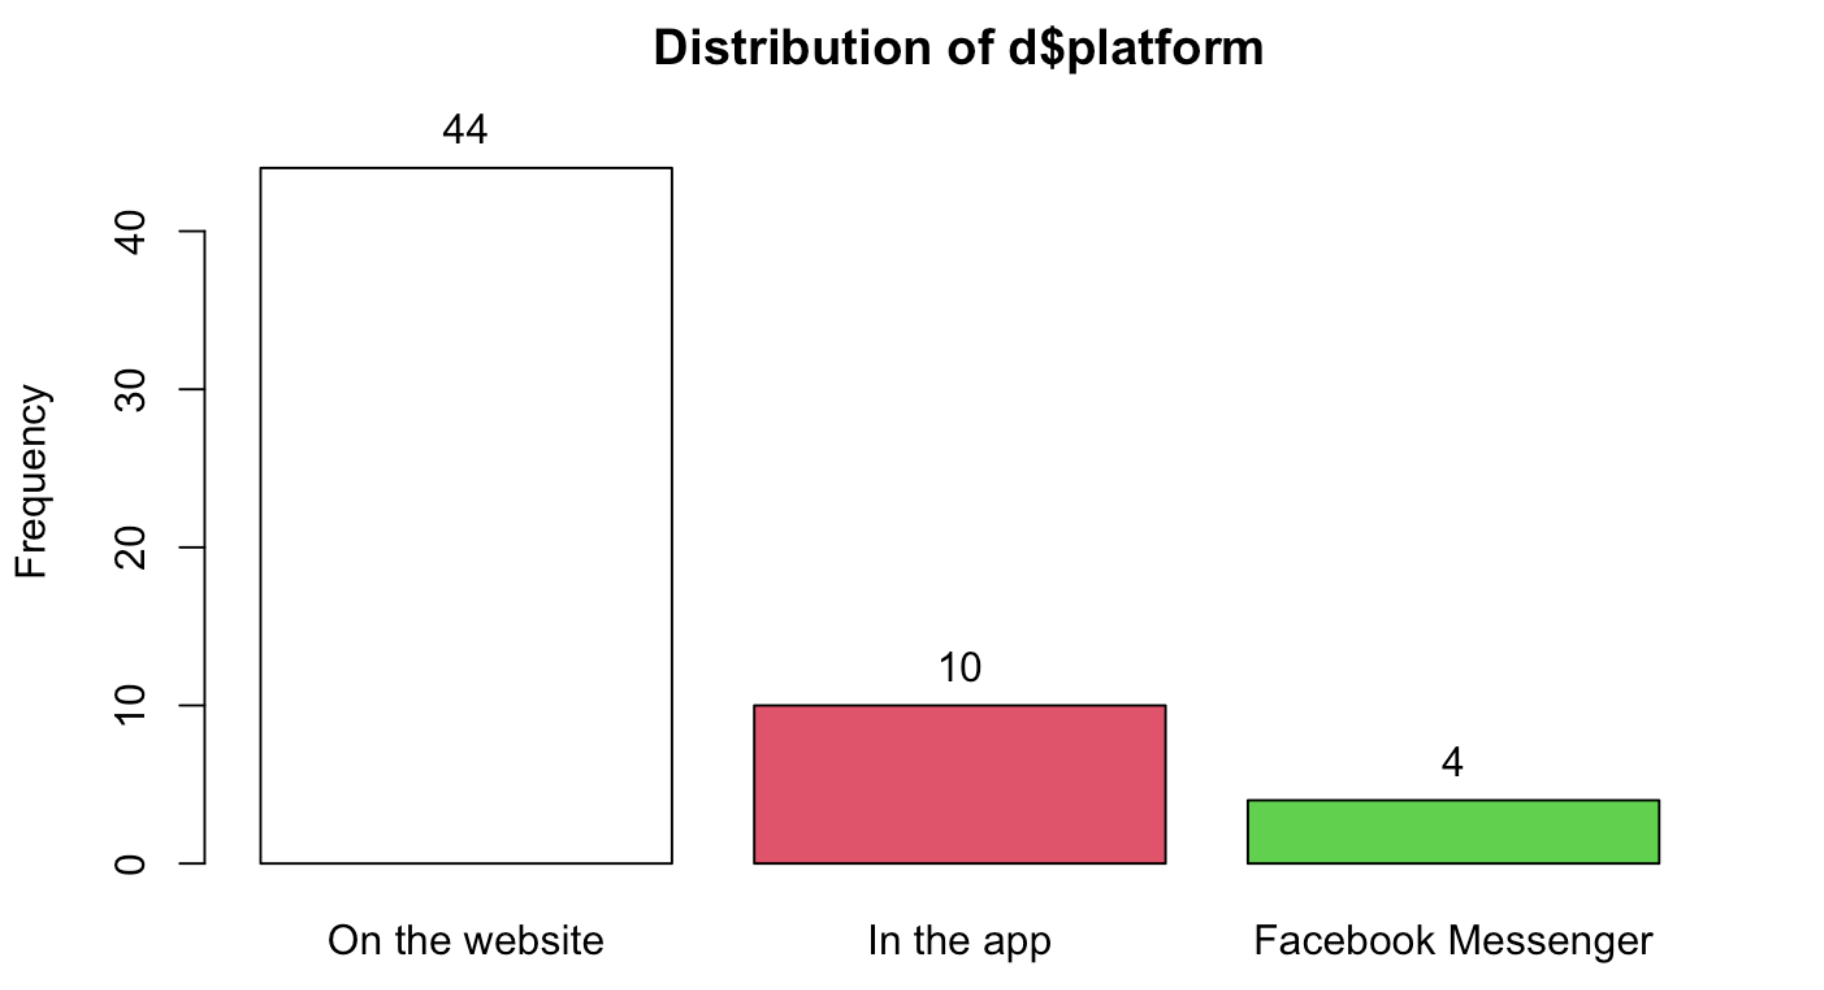
\includegraphics[width=\linewidth]{../LaTeX/Figures/Environments/PlatformPlot.png}
	\caption{The distribution of the platform variable.}\label{fig:platformPlot}
	\endminipage\hfill
	\minipage{0.30\textwidth}
	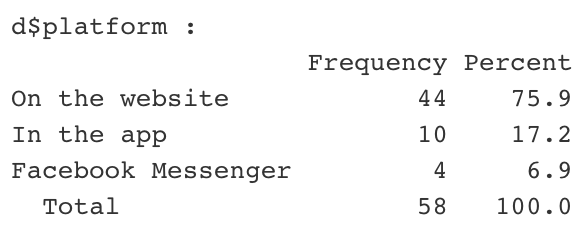
\includegraphics[width=\linewidth]{../LaTeX/Figures/Environments/PlatformFreq.png}
	\caption{A frequency table of all the entries' used platform to interact with the chatbot.}\label{fig:platformFreq}
	\endminipage\hfill
\end{figure}

\subsection{Comparative Study}
\subsubsection{Business view (interviews)}
\myparagraph{1. The current state of the customer service chatbot}
\ul{Task categories}\\
Proximus has a chatbot where the main focus is on support, they try to help people who have not found enough information on the FAQ page or the help center. It was mentioned that the chatbot received specific questions about product and subscription information, then information flows were added that can also answer this, but this is only in a limited form. Later on, they want to develop this further into a proactive salesman with the aim of offering the best action or promotion. Complaints are forwarded by the bot directly to a live agent.\\
\break
Telenet's bot is limited, it only focuses on answering FAQs that are mostly about technical aspects and subscriptions. Telenet used to have two chatbots, which were AskHugo and AskPlay. AskHugo was a bot that tried to convince customers to buy a Hugo subscription, AskPlay gave recommendations on which movies/series to watch. However, both chatbots were shut down because the \acrshort{roi} was too low.\\
\break
T-Mobile\footnote{T-Mobile has merged with Tele2 since January 2019. The Tele2 brand has continued to exist but is therefore a part of T-Mobile. The management of Tele2's chatbot is also done by T-Mobile, these chatbots both use the same underlying system so both chatbots have the same operations.} is offering an extended bot in which customers can ask professional FAQs and purchase add-ons including video services and Deezer (web-streaming service for music). The chatbot can also guide the customer in choosing the right subscription or device. In this way, T-Mobile tries to keep as much "trivial" work away from the physical agents, because the explicit purchase of a specific subscription/device is only done through them. Complaints are also partly handled by the bot, it will always ask if the customer has already spoken to an employee about this, if this has already happened, then the chatbot will give the right procedure to file a complaint.\\
\break
KPN offers a chatbot that also focuses on the complete handling of FAQs. In the case of complaints, the customer is redirected to a live chat; the bot's only function here is to ask for the customer's details so that the physical agent no longer has to do this. Selling products and services is not offered in the bot because that is not yet technically possible, the bot only serves as a proactive assistant, if the customer has been in the shop for a while, the bot will ask the customer if he/she needs help.\\
\break
\ul{Platform}\\
Proximus offers their chatbot via 3 platforms: on the website, in the Proximus app and on Facebook Messenger. Telenet only offers its chatbot through Facebook Messenger, but this is integrated into their website and app. Through Whatsapp, there is also already interaction possible, but this is not a chatbot but just an auto-reply system where you get in touch directly with a live agent. T-Mobile offers their bot through their website and app. There is a difference between these chatbots, on the website all services are offered, but in the application the chatbot is mainly focused on questions about mobile services. If the app chatbot recognises that the customer is asking a question about the "home" services, the customer is redirected to the "home" chatbot on the website. KPN basically only offers their chatbot on their website, but in the app it is also available through a web page built into the application. If the customer then consults the chatbot in the app, this is actually the chatbot on the website.\\
\break
\ul{Supported languages}\\
The Proximus and Telenet bot offers its services in Dutch, French and English. If the Proximus bot is addressed in a different language, the underlying \acrshort{ai} system will recognise that this language is not supported, and the bot will then choose to continue the conversation in English. T-Mobile offers its bot services only in Dutch; if another language is used, the customer is redirected to an agent. KPN's bot is supported in Dutch and English, but the English variant has far fewer functions; it will mainly redirect the customer to the right page on the website or continue the conversation with an agent. According to KPN, there is no need in the Netherlands to offer the chatbot in other languages.\\
\break
\ul{User group}\\
For each company interviewed, it was stated that these specific figures are not monitored or confidential, but other insights were gained. Proximus sees from manual analyses that their chatbot users are widely spread in terms of affinity with technology, they see both very tech-savvy users and people who hardly know which button to press. Proximus' broad customer base explains this spread, as they offer services that are used by young people, adults and the elderly.\\
\break
Telenet especially sees that their bot users are young people and adults up to 40 years of age, which can be explained by the fact that their bot can only be accessed via social media.\\
\break
T-Mobile only has insight into the bot users that have been identified (users who are logged in to their account), from app analyses they see that Tele2's chatbot mainly has younger users, which is also in line with what the brand wants to convey. The users of the T-Mobile bot are older. T-Mobile also anticipates this aspect by adjusting the chat style; in the Tele2 bot, more hashtags and emojis are used, in the T-Mobile bot this is more formal.\\
\break
KPN has no specific idea which age group uses their bot most. According to Justin, it is mainly the older target group, but specific numbers could not be given. KPN uses a neutral chat style in their bot, so they don't want to address a specific age group.\\
\break
\ul{Supported types of questions}\\
For every bot except Telenet, it can be concluded that the yes/no questions are supported. The treatment of the direct and vague is also in the same line in the different bots. Whenever a question is too vague, the bot will continue to ask until the various missing values have been filled in. In the T-Mobile bot, it was mentioned that there is a limit to the number of times that a certain missing value can be queried. If the bot needs to ask a certain number of times before it can provide an answer, the chat will be redirected to a live agent to avoid user frustration, as it was mentioned that it can be frustrating for a customer to get stuck for a long time on a certain question. To address this issue, KPN is using a button where the user can indicate whether they mean something different or have a different question.\\
Telenet's chatbot can't interpret anything, you have to work with the buttons provided by the chatbot.\\
\break

\paragraph{2. The benefits that the company derives from the presence of the
	chatbot}
\ul{Supported services}\\
The Proximus chatbot can retrieve a pincode, show the outstanding invoice amount. It is also possible to request postponement of payment if the amount cannot be paid before the invoice date. The chatbot can retrieve the status of your subscription and services. The purpose of Proximus' chatbot is to offer solutions, not instructions such as "for that task, you can go to this page where we have an explanation for you".\\
\break
Telenet's chatbot is mainly used for support; if certain services need to be carried out, the chatbot will collect the necessary customer information so that it can be further handled by an agent.\\
\break
T-Mobile has a more extensive bot, which can be used to retrieve customer information (customer number, puk code, ...), it can also be used to adjust certain settings, for example if the customer calls a service number and then has to pay extra costs, the user can deactivate this via the bot. It is also possible to buy certain services, even if these are just add-ons like an extra mobile data bundle. Contracts are not handled in the chatbot because the sales department doesn't want to deal with this regarding certain sales strategies. The chatbot also serves as a kind of workforce manager, it will ensure that there is no overload of agents.\\
\break
KPN's chatbot generally offers two overarching services. Firstly, it serves as a work preparer for the agents, namely it tries to make the conversation with the agents shorter by retrieving general information before the conversation with the agent starts. Secondly, the chatbot will also serve as a kind of guide that will lead the customer to the right page on the website so that they can find their answer there.\\
\break
\ul{Reduction of employee workload}\\
Proximus could not share specific data because this was too confidential, but they did say that not everything in customer service was covered, so for some issues customers were put straight through to an employee. Telenet also did not have the data to answer this question with explicit figures. The chatbot reduces the workload, but the impact is not great because the knowledge of the chatbot is still limited. T-Mobile's chatbot is unable to complete its task independently in about 25\% of cases, which can be explained by poor language use by the customer or the complexity and specificity of the question. KPN's chatbot is not capable of answering the question/task in about 50\% of the cases. This is not always because the bot does not have enough knowledge to answer the question; for some services, such as cancelling subscriptions or complaints, the customer is always referred to a member of staff. It is estimated that about a quarter (25\%) of the agents' work is taken over by the chatbot.\\
\break
\ul{Customer's willingness to use chatbot}\\
The willingness to use the chatbot is examined by each company on the basis of feedback, with feedback one must also take into account voluntary response bias, customers who are not satisfied with certain services will give feedback more quickly than others.\\ 
\break
At Proximus the satisfaction lies in both camps, there are customers who are very satisfied with the chatbot, but there are also customers who think it is very bad, again we have to take into account bias. Proximus could not share an overall satisfaction level.\\
\break
Telenet has already done analyses in which they measure that 65\% of chatbot users are willing to go through the whole flow of a chatbot, this means that 65\% of the users who start a conversation also complete it. The reason why the remaining 30-35\% drop out is explained by a bad previous experience with a similar chatbot.\\
\break
T-Mobile asks their customers for feedback after a conversation with a chatbot, and here too the voluntary response bias comes to the fore. Analyses showed that the majority of responses ultimately had to call an agent to solve their problem. What T-Mobile also does to gain more insight into their customers is to work with personas. These are linked to certain possible customer profiles where they try to map out the chatbot requirements of the customer.\\
\break
KPN also uses feedback to see if the customer is satisfied with the chatbot, here too there is bias. It was estimated that about 20\% of the customers communicating with chatbot would like to communicate with an agent. The number of direct calls (telephone) to a physical agent would be up higher, to an order of about 10, than with the chatbot. This means that there are 10 times more calls than chats.\\
\break
\ul{Negative influences}\\
Proximus sees mainly negative influences in the form of customers who are frustrated. The frustration arises mainly when the chatbot does not understand the customer properly and goes the wrong way, this will make this type of customer unwilling to use the chatbot in the future. Again, customers who are already frustrated by services that don't work properly (bad wifi connection) should be taken into account, if these customers then come into contact with a chatbot it won't help their mood.\\
\break
Telenet experiences similar scenarios, it was further explained that it can sometimes be frustrating for customers to switch to a new platform, namely from 100\% helpdesk to a chatbot. According to Ms Portolani, some customers expect that a chatbot can interpret in the same way as an agent, and thus in an empathic way.\\
\break
T-Mobile has the same negative aspects as Proximus, they try to solve this by applying a limited form of sentiment analysis. If they measure that a customer is communicating in a frustrated way, they will forward this customer to an agent.\\
\break
At KPN, different metrics are used. For instance, the \gls{nps} measures the extent to which customers would recommend the company to acquaintances. The \acrshort{ces} measures how much effort it took to find the answer to the question. The final metric measured is the \acrshort{gcr}, which tells more about how well the customer was helped. The results of these metrics were not shared due to confidential information.\\
\break

\myparagraph{3. The business value (revenue, reduced costs) realised by the chatbot}
\ul{Increased revenue}\\
Proximus does not yet see any direct revenue from the model, as the bot is very expensive and a concrete \acrshort{roi} has not yet been determined. Concrete figures could not be given because they are difficult to calculate, there are many factors that can influence it. The chatbot indirectly ensures that Proximus has to spend less on physical agents because they are less needed.\\
\break
At Telenet, too, there is no picture of how much extra revenue was caused by the chatbot, but here too, the fact that fewer costs had to be spent on physical agents was mentioned.\\
\break
At T-Mobile and KPN, no concrete figures were disclosed either, because this is not measured. In both cases, cost reduction in the area of employees was addressed. It can therefore be concluded that with each of the chatbots, extra business value is created because fewer costs have to be spent on physical agents.\\
\break
\ul{Availability}\\
Every chatbot that was questioned is available 24/7, but there is a difference in the handling of questions that cannot be solved by the chatbot during non-opening hours.
With the Proximus chatbot, the follow-up depends on whether the user has identified himself. On social media a follow-up is possible, on the website and in the application this is also possible if the user has authenticated himself. With Telenet's chatbot, the question is tracked anyway because all communication is done through social media. With the chatbots of T-Mobile and KPN, the conversation is not tracked, so the customer will have to consult the chatbot again during opening hours if the question cannot be answered.\\
\break
\ul{Costs \& cost items}\\
In none of the interviews was it possible to put a specific figure on the total cost of the chatbots, but the biggest cost items were always indicated.\\
\break
With the Proximus chatbot, the costs depend mainly on the platform used and the size of the chatbot; the size of the bot depends on the number of questions/scenarios that are added. The biggest cost items are the standard amount that has to be paid each time the \acrshort{nlp} is triggered. This is calculated per incoming chat and amounts to about 1 cent. There is also a team behind the chatbot that consists of in-house frontend and backend developers and configuration/conversation designers. These last two are mainly done via consultancy and cost about € 400/day. For the rest, an \acrshort{nlp} trainer and engineer are needed to train and correct the \acrshort{nlp}.\\  
\break
At Telenet, a pay-as-you-go service is implemented. Specific figures about this cost were not shared due to confidential information. The other biggest cost items are the hosting of the chatbot and the team behind the development. Currently, the team includes a data scientist, developer, functional analyst and a product owner. It was reported that most of the cost goes to the team.\\
\break
T-Mobile runs its chatbot in the cloud, which means they have to pay a significant amount of running costs. T-Mobile also uses Dialogflow from Google, which is a tool that contains a \acrshort{cms} and where you can apply \acrshort{ai}. The running costs also consist of a classification \acrshort{api}, database operations and running the engines to keep everything working. The largest part of the costs is also in the team behind the bot, which consists of two developers, full-stack developers from India (quantity unknown), two \acrshort{ai} trainers and two conversation designers.\\
\break
The costs at KPN are in the same line as at T-Mobile, although there is less specific knowledge about how the cost items are distributed.\\
\break
\myparagraph{4. The company’s future vision of the chatbot}
\ul{Focal points for the future}\\
Proximus' view for the future was mostly confidential. They did mention that they are looking further into voice control, which would be the next channel they would like to capitalise on. They are also looking at applying sentiment analysis within the current chatbot to improve it even further. In general, they are looking to automate their services more and more and to be stronger in terms of conversation. They also want to take the buttons out of the chatbot, the goal is really to be as conversational as possible to really feel like you are not talking to a robot, even though they don't want to fake that they are talking to a real human being either. They are also looking at computer vision, for example, if a picture of an invoice is sent, the chatbot can automatically recognise the different elements. In the long term, they are also looking at integrating the bot with Alexa, Google home, etc.\\
\break
Telenet is currently working on a platform in which the chatbot can take on many more tasks and answer questions independently. Afterwards, sentiment analysis will be added. They will also look to brand this chatbot so that it becomes known to its future users. They also focus on automating certain things the agents work with, they want to add text prediction so when the agent starts typing they will automatically prefill things so the agent doesn't have to type everything themselves..\\
\break
T-Mobile wants to offer the chatbot more proactively in the future, this means that they will offer the chatbot via e-mail and on a more prominent place on the website. They are also looking to offer the chatbot in multiple languages by using a translate API that allows both parties to communicate in their own language. They are also working on asynchronous messaging, which means that if it is necessary to chat with an agent, no synchronous connection is needed, and the flow of the chat will continue exactly as it started with the chatbot. The latter will also ensure that customers do not need to send their question again if they have consulted the chatbot outside of helpdesk opening hours.\\
\break
KPN's vision for the future is to be available in more places, they want to be where the customers are the most, this translates into a presence on social media such as Facebook Messenger and Whatsapp. Furthermore, they want to harmonise the entire communication with the customer, if the customer would send them via Whatsapp, then they want to be aware of this conversation if the customer contacts them via another platform.\\
\break
\ul{Additional chatbot-features}\\
The chatbots of Proximus, T-Mobile and KPN are AI-based to classify the question or statement of the customer, once this is classified a rules-based approach is used. The Telenet bot is the only one that is 100\% rules-based.\\
\break
\ul{Source of knowledge to improve chatbot}\\
Different methodologies are used to find out what the most relevant scenarios should be in the chatbot. Proximus uses benchmarking, marketing studies, check-ins with other companies, research in papers and participation in many conferences to gather extra information on what the relevant topics their chatbot should respond to, are.\\
\break
Telenet mainly uses data analysis, they also look at the experience of their agents.\\
\break
T-Mobile also uses data analysis, every conversation in the chatbot is logged, so they can further query this to gather information on specific topics. The customer feedback on these conversations is also taken into account. In the conversations that went well, they look for common features so that they can be further standardised. In the bad conversations, they look for aspects on which they can further improve.\\
\break
At KPN, data analysis is also the main focus. Just like T-Mobile, they continuously review how they can improve the conversations.\\
\break
\subsubsection{Customer view (survey)}
In this part, a comparison will be drawn between the different companies in accordance to the business interview and gathered data in the survey. Because Orange, T-Mobile/Tele2 and KPN didn't get enough responses to be viewed on their own, these three providers will be grouped together in the group 'others'.\\
\break
Next up, the task categories. Because the interview showed that chatbots aren't yet equipped to deal with both complaints as well as sales questions, these two won't be included in the comparative study. For personal questions, there aren't enough entries to view this as it's own category. The focus will thus be on FAQ questions.\\
\break
All graphs will be presented as follows: Telenet on the left, Proximus in the middle and the others on the right.\\
\break
\ul{Attribute 1: Execute the requested task}\\
\break
When looking at how the chatbots performed when solving a task, both Telenet and Proximus seem to have a split customer base where around 50\% is happy and 50\% isn't. When looking at the others, there is a clear happiness about how the chatbot performed.\\
\begin{figure}[!htb]
	\minipage{0.32\textwidth}
	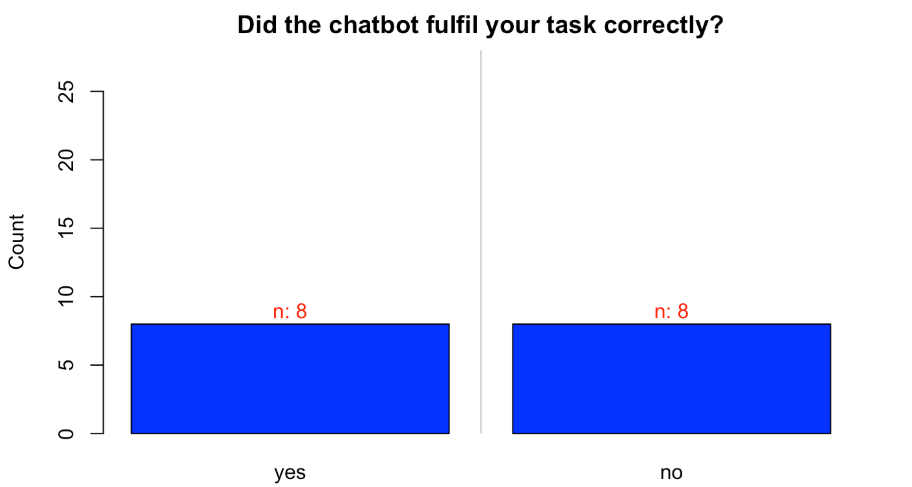
\includegraphics[width=\linewidth]{../LaTeX/Figures/Comparative/Q1T.png}
	\caption{Bar chart of the responses for Telenet about the functional question for attribute 1, question 1.}\label{fig:Q1T}
	\endminipage\hfill
	\minipage{0.32\textwidth}
	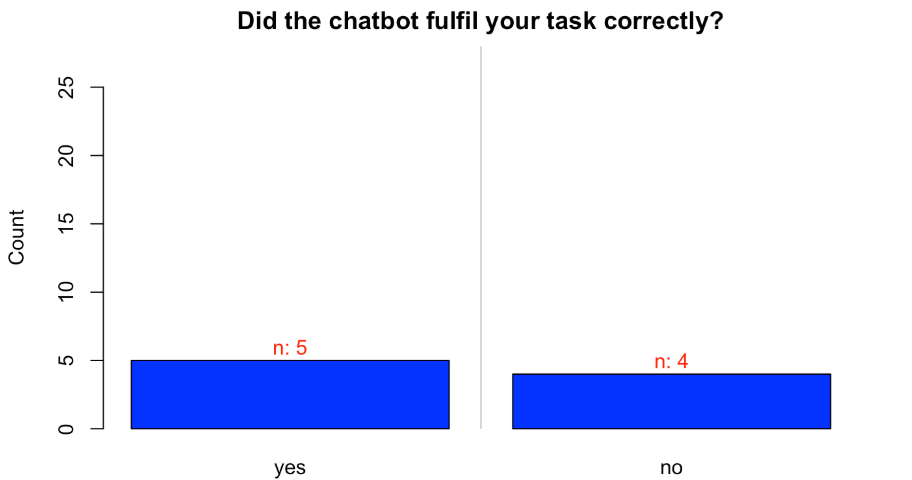
\includegraphics[width=\linewidth]{../LaTeX/Figures/Comparative/Q1P.png}
	\caption{Bar chart of the responses for Proximus about the functional question for attribute 1, question 1.}\label{fig:Q1P}
	\endminipage\hfill
	\minipage{0.32\textwidth}
	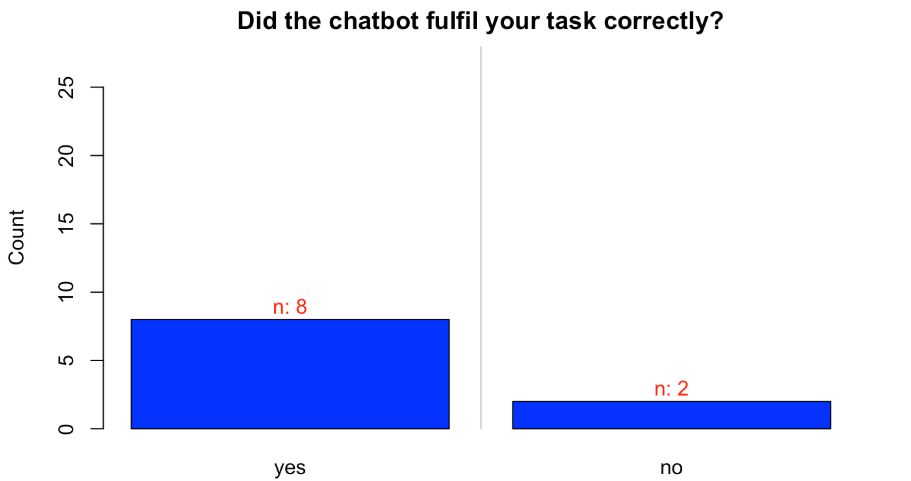
\includegraphics[width=\linewidth]{../LaTeX/Figures/Comparative/Q1O.png}
	\caption{Bar chart of the responses for the others about the functional question for attribute 1, question 1.}\label{fig:Q1O}
	\endminipage\hfill
\end{figure}
Looking at the counter part of the previous question, there is even more discontent with Proximus. The results for Telenet and the others confirm the previous findings.\\
\begin{figure}[!htb]
	\minipage{0.32\textwidth}
	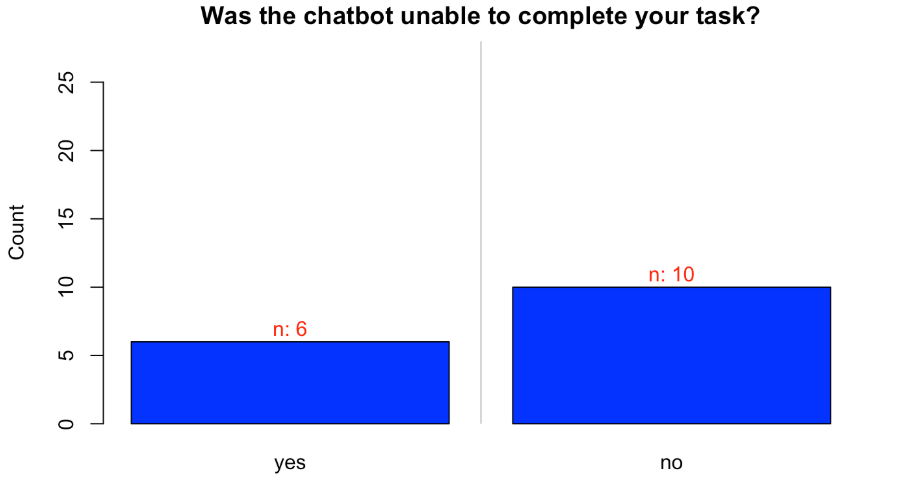
\includegraphics[width=\linewidth]{../LaTeX/Figures/Comparative/DQ1T.png}
	\caption{Bar chart of the responses for Telenet about the dysfunctional question for attribute 1, question 1.}\label{fig:DQ1T}
	\endminipage\hfill
	\minipage{0.32\textwidth}
	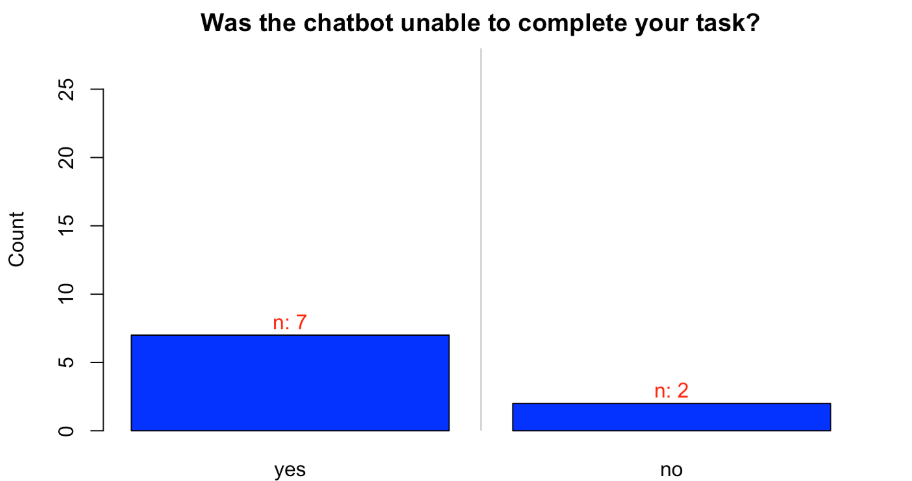
\includegraphics[width=\linewidth]{../LaTeX/Figures/Comparative/DQ1P.png}
	\caption{Bar chart of the responses for Proximus about the dysfunctional question for attribute 1, question 1.}\label{fig:DQ1P}
	\endminipage\hfill
	\minipage{0.32\textwidth}
	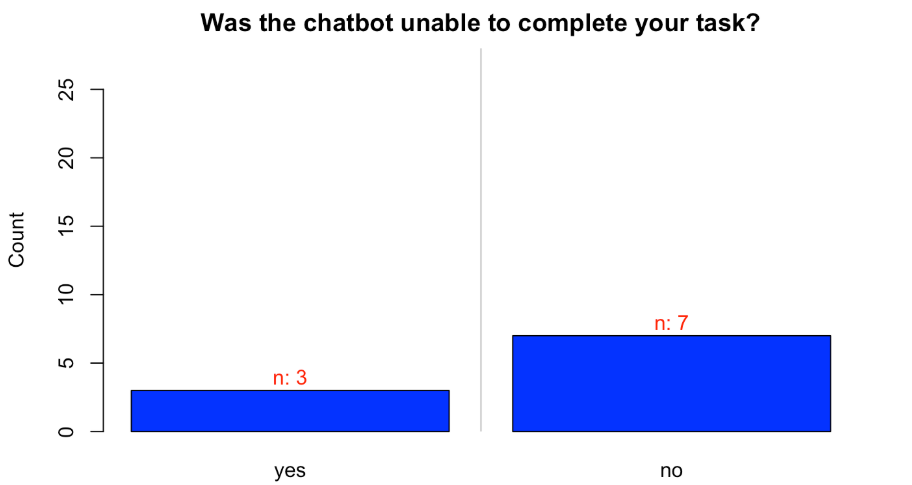
\includegraphics[width=\linewidth]{../LaTeX/Figures/Comparative/DQ1O.png}
	\caption{Bar chart of the responses for the others about the dysfunctional question for attribute 1, question 1.}\label{fig:DQ1O}
	\endminipage\hfill
\end{figure}
\break
A second aspect researched is whether the chatbot needed help from a human agent to complete it's task. Looking at the results, there again is almost a 50-50 split for Telenet and Proximus whereas the others did better again.\\
\begin{figure}[!htb]
	\minipage{0.32\textwidth}
	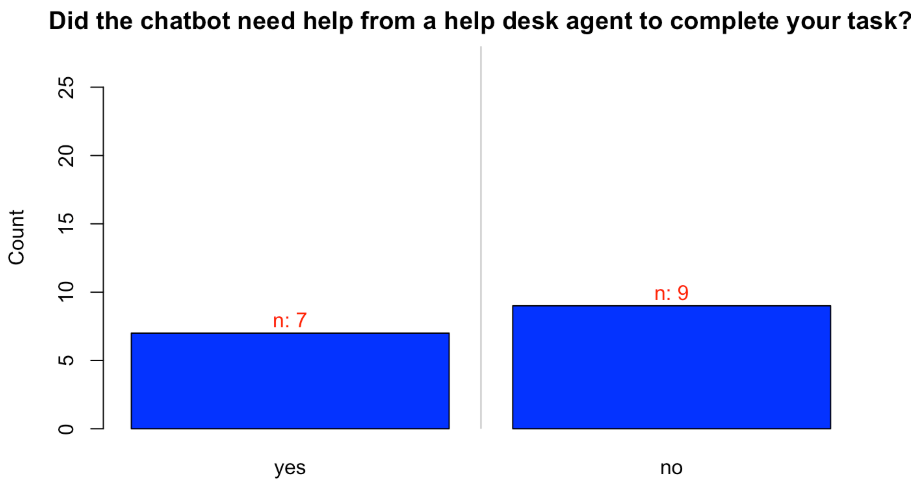
\includegraphics[width=\linewidth]{../LaTeX/Figures/Comparative/Q1Tb.png}
	\caption{Bar chart of the responses for Telenet about the functional question for attribute 1, question 2.}\label{fig:Q1Tb}
	\endminipage\hfill
	\minipage{0.32\textwidth}
	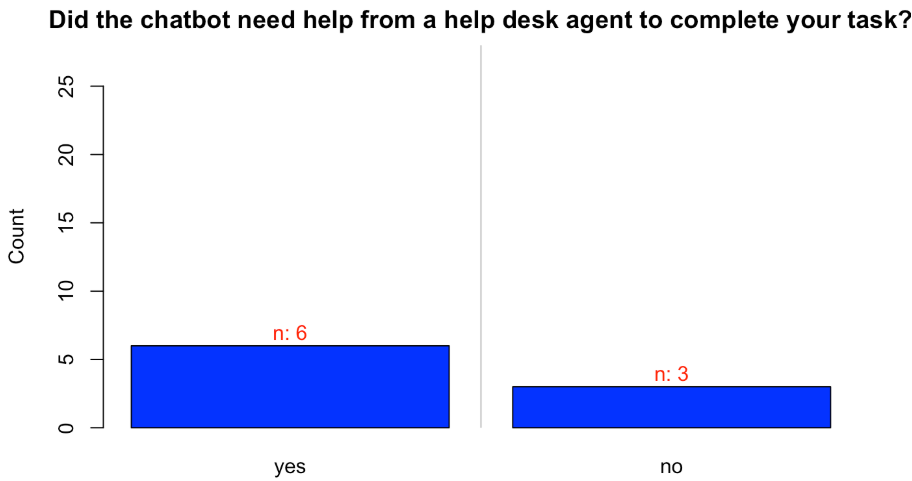
\includegraphics[width=\linewidth]{../LaTeX/Figures/Comparative/Q1Pb.png}
	\caption{Bar chart of the responses for Proximus about the functional question for attribute 1, question 2.}\label{fig:Q1Pb}
	\endminipage\hfill
	\minipage{0.32\textwidth}
	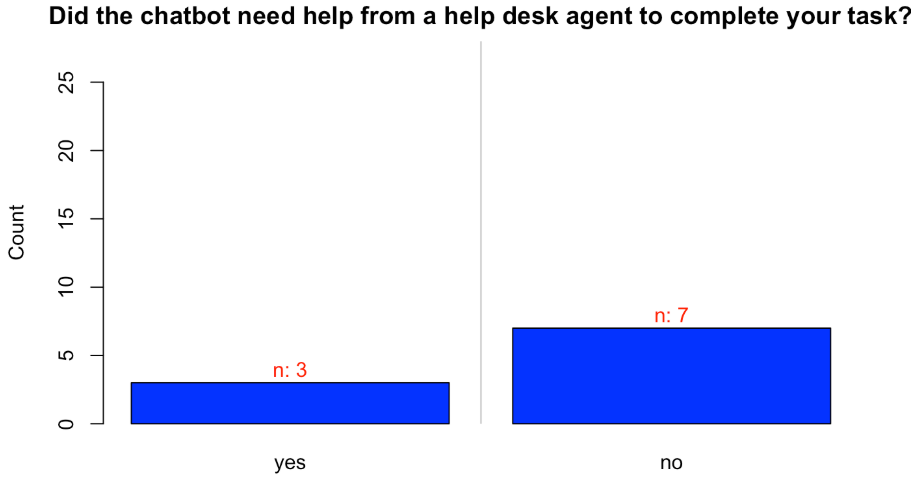
\includegraphics[width=\linewidth]{../LaTeX/Figures/Comparative/Q1Ob.png}
	\caption{Bar chart of the responses for the others about the functional question for attribute 1, question 2.}\label{fig:Q1Ob}
	\endminipage\hfill
\end{figure}
The dysfunctional version of the previous question confirms these findings for Telenet, Proximus and the others.\\
\begin{figure}[!htb]
	\minipage{0.32\textwidth}
	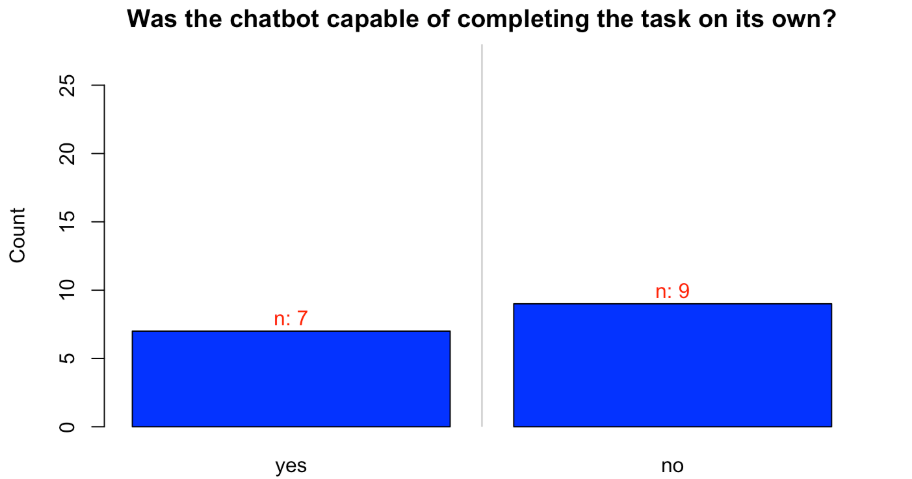
\includegraphics[width=\linewidth]{../LaTeX/Figures/Comparative/DQ1Tb.png}
	\caption{Bar chart of the responses for Telenet about the dysfunctional question for attribute 1, question 2.}\label{fig:DQ1Tb}
	\endminipage\hfill
	\minipage{0.32\textwidth}
	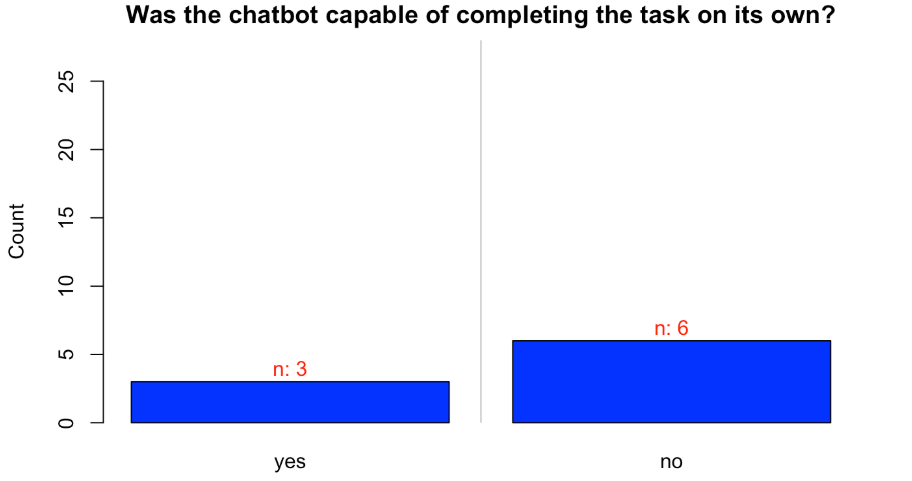
\includegraphics[width=\linewidth]{../LaTeX/Figures/Comparative/DQ1Pb.png}
	\caption{Bar chart of the responses for Proximus about the dysfunctional question for attribute 1, question 2.}\label{fig:DQ1Pb}
	\endminipage\hfill
	\minipage{0.32\textwidth}
	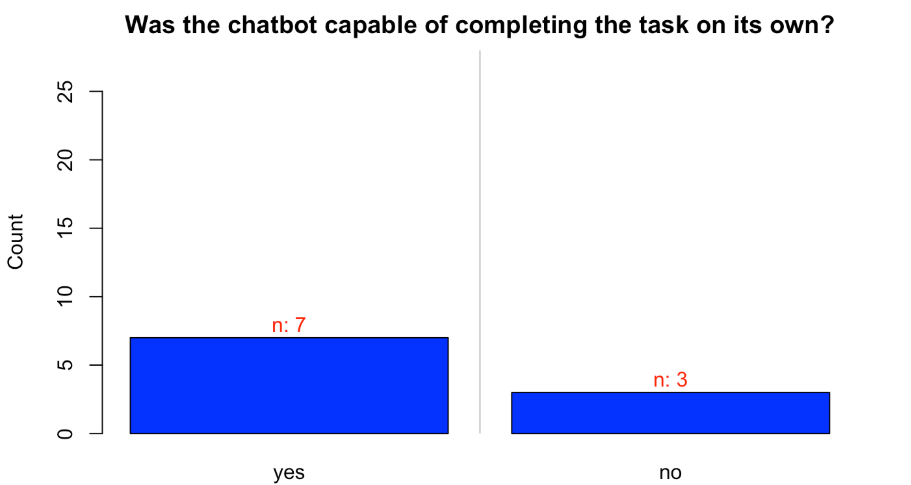
\includegraphics[width=\linewidth]{../LaTeX/Figures/Comparative/DQ1Ob.png}
	\caption{Bar chart of the responses for the others about the dysfunctional question for attribute 1, question 2.}\label{fig:DQ1Ob}
	\endminipage\hfill
\end{figure}
\break
A third question to gauge the capabilities of the chatbot to execute the requested task was about the expectations of the chatbot and if it lived up to them. The results show that the chatbot mostly lived up to expectations, even though it couldn't solve the task it was given.\\
\begin{figure}[!htb]
	\minipage{0.32\textwidth}
	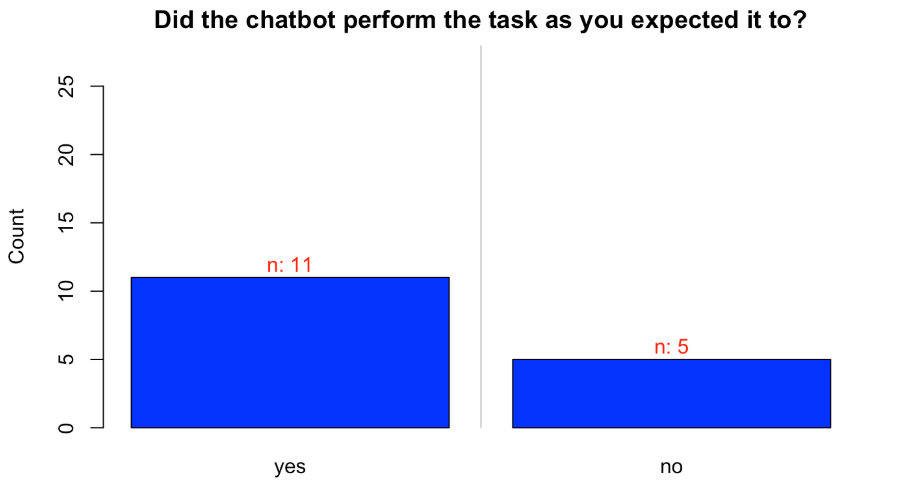
\includegraphics[width=\linewidth]{../LaTeX/Figures/Comparative/Q1Tc.png}
	\caption{Bar chart of the responses for Telenet about the functional question for attribute 1, question 3.}\label{fig:Q1Tc}
	\endminipage\hfill
	\minipage{0.32\textwidth}
	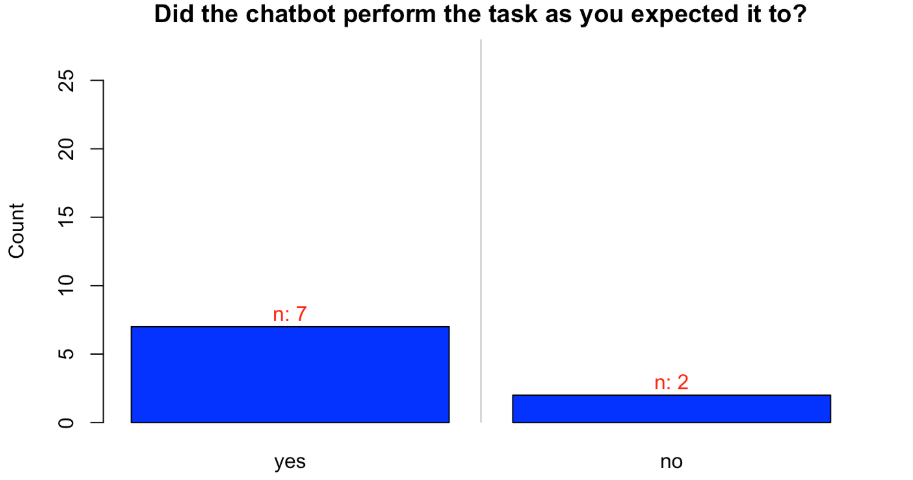
\includegraphics[width=\linewidth]{../LaTeX/Figures/Comparative/Q1Pc.png}
	\caption{Bar chart of the responses for Proximus about the functional question for attribute 1, question 3.}\label{fig:Q1Pc}
	\endminipage\hfill
	\minipage{0.32\textwidth}
	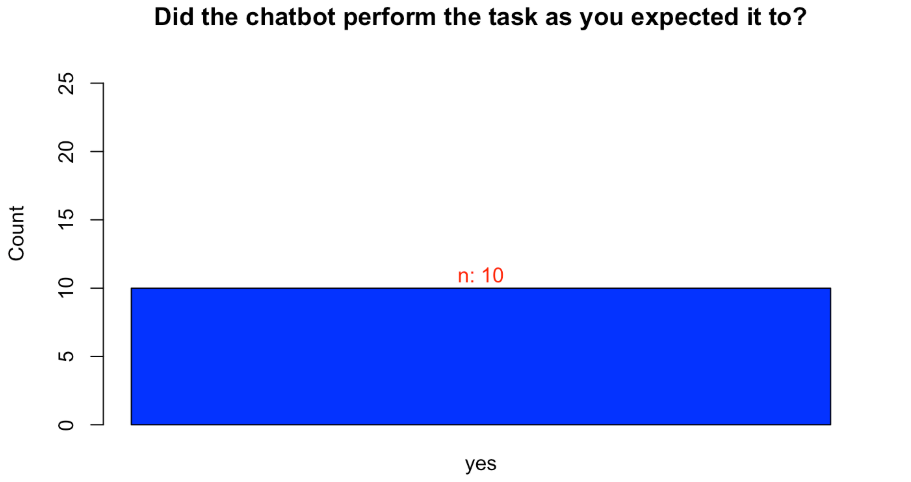
\includegraphics[width=\linewidth]{../LaTeX/Figures/Comparative/Q1Oc.png}
	\caption{Bar chart of the responses for the others about the functional question for attribute 1, question 3.}\label{fig:Q1Oc}
	\endminipage\hfill
\end{figure}
A fourth and final question asked if the user could solve the problem after interacting with the chatbot. For Proximus, there was some pushback but for Telenet and the others, the majority voted yes.\\
\begin{figure}[!htb]
	\minipage{0.32\textwidth}
	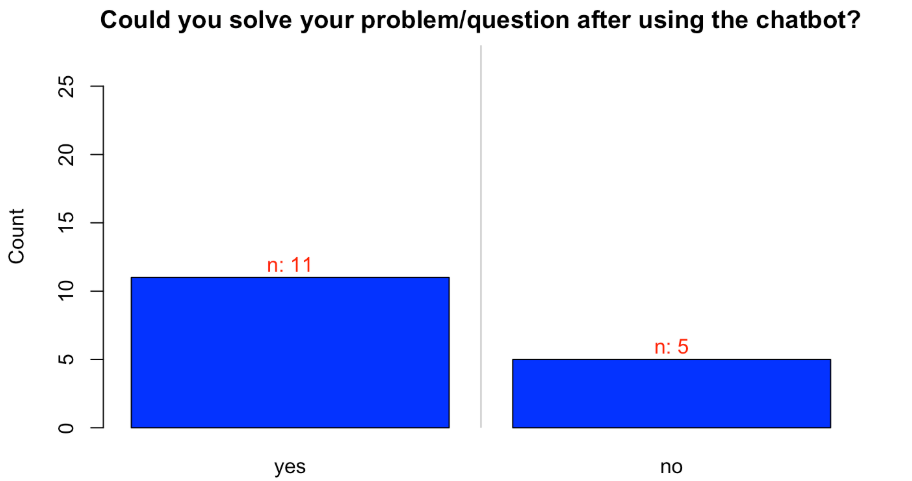
\includegraphics[width=\linewidth]{../LaTeX/Figures/Comparative/DQ1Tc.png}
	\caption{Bar chart of the responses for Telenet about the dysfunctional question for attribute 1, question 4.}\label{fig:DQ1Tc}
	\endminipage\hfill
	\minipage{0.32\textwidth}
	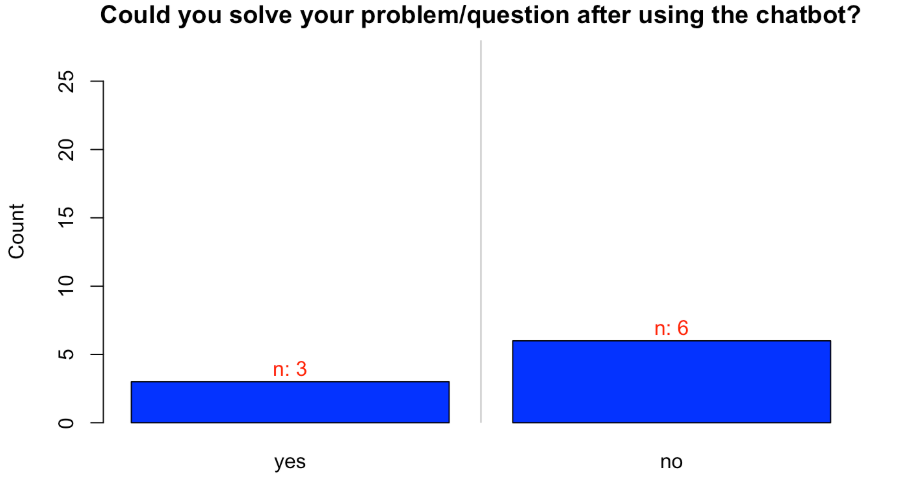
\includegraphics[width=\linewidth]{../LaTeX/Figures/Comparative/DQ1Pc.png}
	\caption{Bar chart of the responses for Proximus about the dysfunctional question for attribute 1, question 4.}\label{fig:DQ1Pc}
	\endminipage\hfill
	\minipage{0.32\textwidth}
	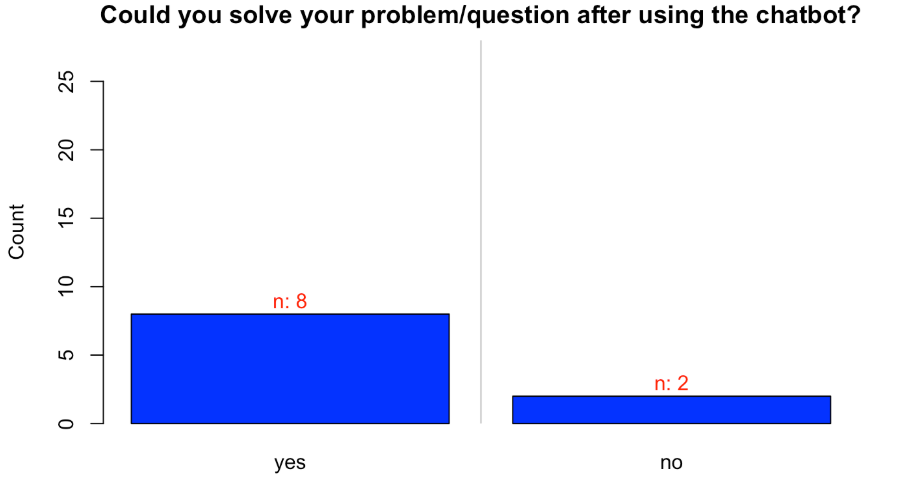
\includegraphics[width=\linewidth]{../LaTeX/Figures/Comparative/DQ1Oc.png}
	\caption{Bar chart of the responses for the others about the dysfunctional question for attribute 1, question 4.}\label{fig:DQ1Oc}
	\endminipage\hfill
\end{figure}
\break
\ul{Attribute 2: Number of services}\\
\break
Attribute 2 looked at the services available and delivered by the chatbot in comparison to a human agent. The responses about whether a chatbot delivers a better service than a human agent were for both Telenet and the others an outstanding no whereas for Proximus, the votes were more divided. For Proximus, there is almost a 50-50 split.\\
\begin{figure}[!htb]
	\minipage{0.32\textwidth}
	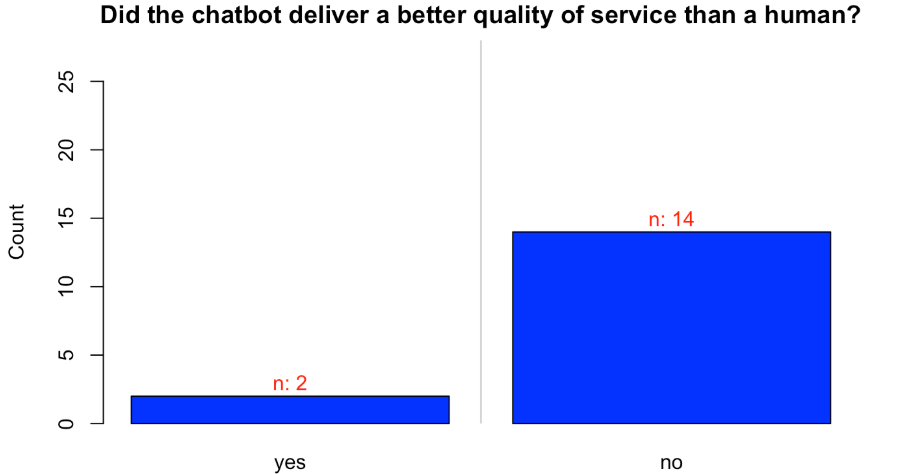
\includegraphics[width=\linewidth]{../LaTeX/Figures/Comparative/Q2T.png}
	\caption{Bar chart of the responses for Telenet about the functional question for attribute 2.}\label{fig:Q2T}
	\endminipage\hfill
	\minipage{0.32\textwidth}
	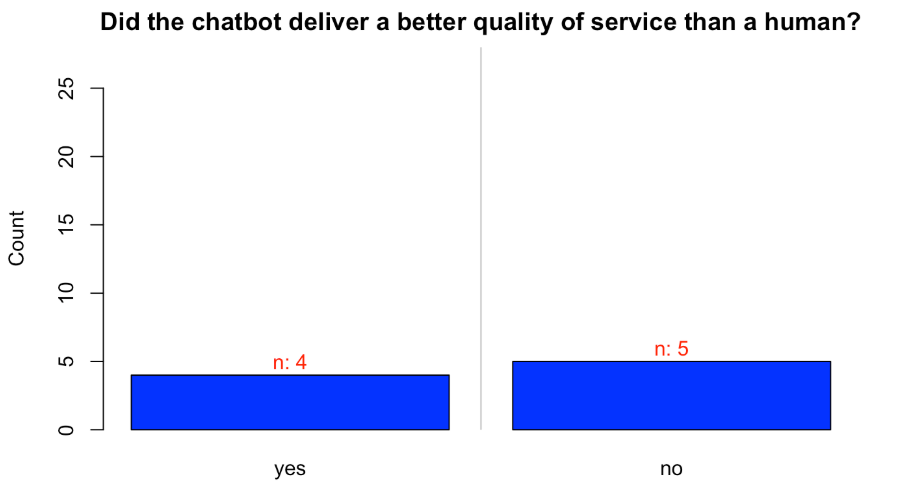
\includegraphics[width=\linewidth]{../LaTeX/Figures/Comparative/Q2P.png}
	\caption{Bar chart of the responses for Proximus about the functional question for attribute 2.}\label{fig:Q2P}
	\endminipage\hfill
	\minipage{0.32\textwidth}
	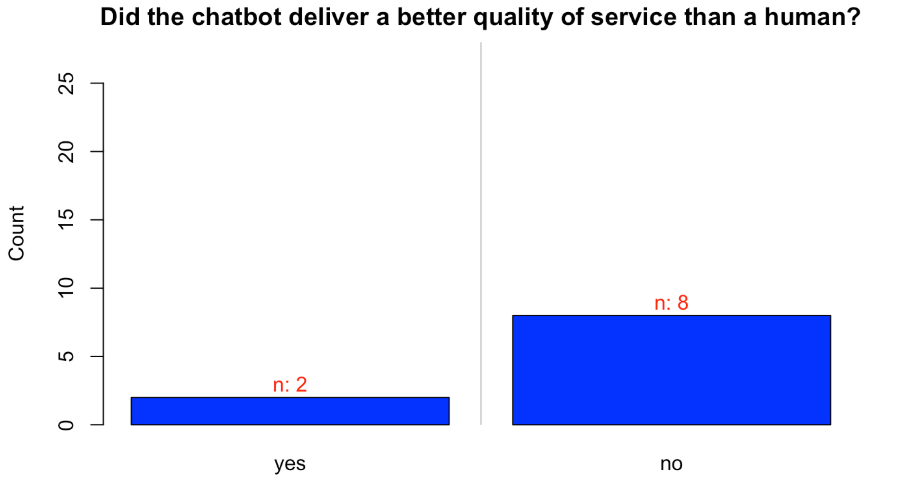
\includegraphics[width=\linewidth]{../LaTeX/Figures/Comparative/Q2O.png}
	\caption{Bar chart of the responses for the others about the functional question for attribute 2.}\label{fig:Q2O}
	\endminipage\hfill
\end{figure}
When asked whether the service delivered by a human was of better quality, the responses for each group were almost always yes.\\
\begin{figure}[!htb]
	\minipage{0.32\textwidth}
	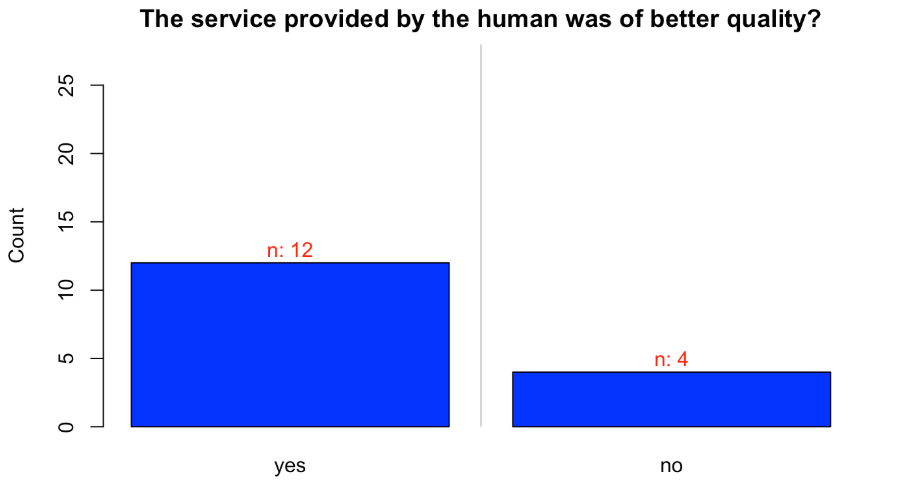
\includegraphics[width=\linewidth]{../LaTeX/Figures/Comparative/DQ2T.png}
	\caption{Bar chart of the responses for Telenet about the dysfunctional question for attribute 2.}\label{fig:DQ2T}
	\endminipage\hfill
	\minipage{0.32\textwidth}
	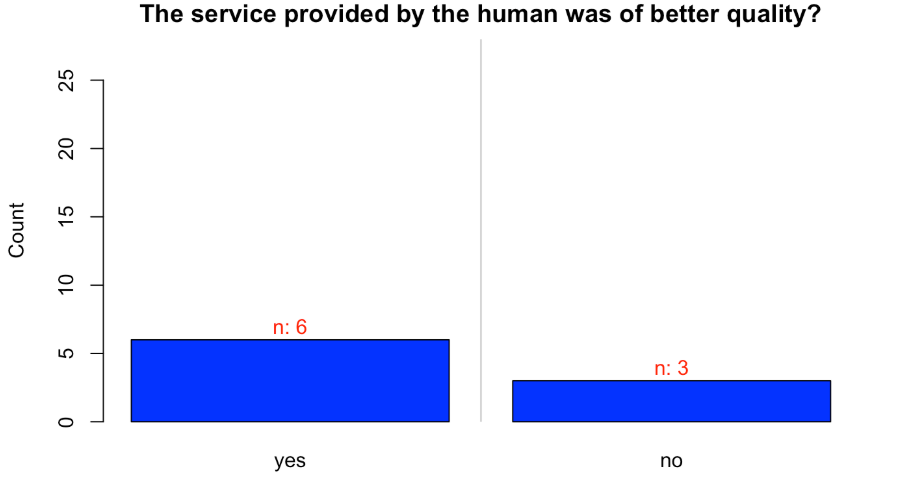
\includegraphics[width=\linewidth]{../LaTeX/Figures/Comparative/DQ2P.png}
	\caption{Bar chart of the responses for Proximus about the dysfunctional question for attribute 2.}\label{fig:DQ2P}
	\endminipage\hfill
	\minipage{0.32\textwidth}
	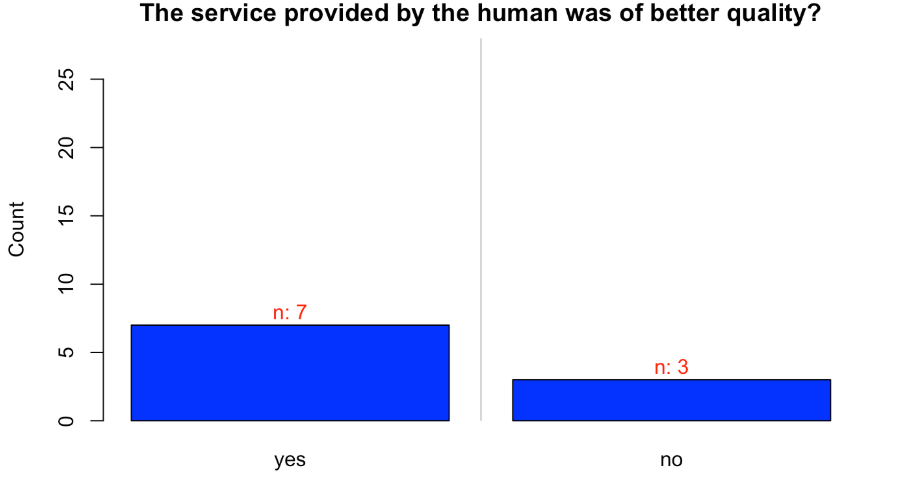
\includegraphics[width=\linewidth]{../LaTeX/Figures/Comparative/DQ2O.png}
	\caption{Bar chart of the responses for the others about the dysfunctional question for attribute 2.}\label{fig:DQ2O}
	\endminipage\hfill
\end{figure}
\break
\ul{Attribute 3: Breadth of knowledge}\\
\break
Attribute 3 handles breadth of knowledge: how knowledgeable is the chatbot. When presented with the question "Did the chatbot contain enough knowledge to help with your problem", the responses for each group differ a lot. For Telenet, there again is about a 50-50 split. Proximus on the other hand is mostly negative. This contrasts the other group where the responses were mainly positive.\\
\begin{figure}[!htb]
	\minipage{0.32\textwidth}
	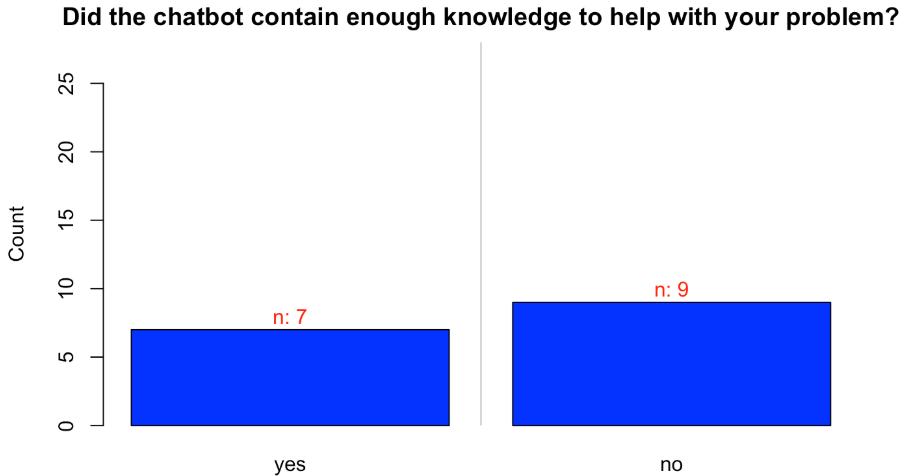
\includegraphics[width=\linewidth]{../LaTeX/Figures/Comparative/Q3T.png}
	\caption{Bar chart of the responses for Telenet about the functional question for attribute 3, question 1.}\label{fig:Q3T}
	\endminipage\hfill
	\minipage{0.32\textwidth}
	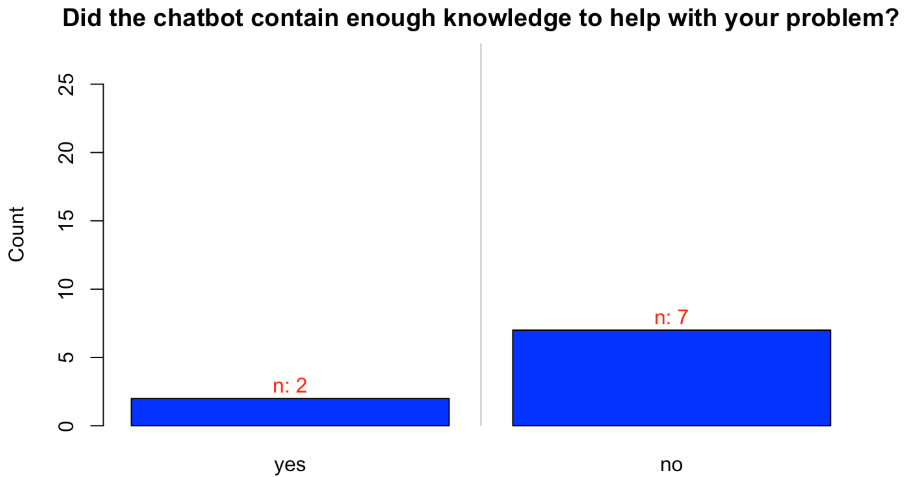
\includegraphics[width=\linewidth]{../LaTeX/Figures/Comparative/Q3P.png}
	\caption{Bar chart of the responses for Proximus about the functional question for attribute 3, question 1.}\label{fig:Q3P}
	\endminipage\hfill
	\minipage{0.32\textwidth}
	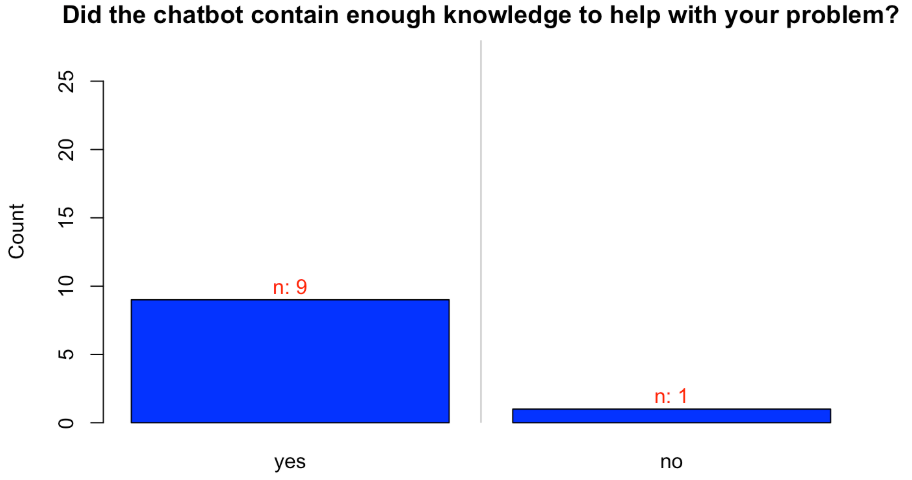
\includegraphics[width=\linewidth]{../LaTeX/Figures/Comparative/Q3O.png}
	\caption{Bar chart of the responses for the others about the functional question for attribute 3, question 1.}\label{fig:Q3O}
	\endminipage\hfill
\end{figure}
When asking the inverse, namely: "The chatbot didn't know what he was talking about", the answers provided were more streamlined to be mostly negative. In other words, the chatbot knows what he is talking about.\\
\begin{figure}[!htb]
	\minipage{0.32\textwidth}
	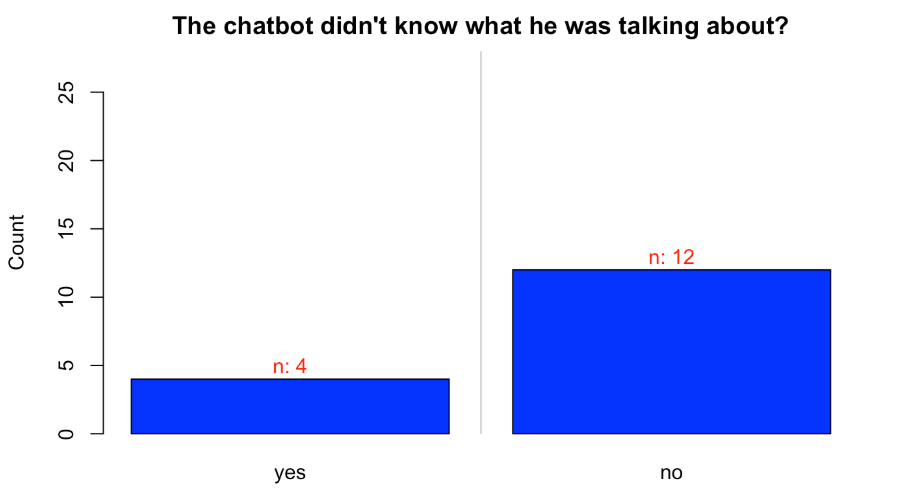
\includegraphics[width=\linewidth]{../LaTeX/Figures/Comparative/DQ3T.png}
	\caption{Bar chart of the responses for Telenet about the dysfunctional question for attribute 3, question 1.}\label{fig:DQ3T}
	\endminipage\hfill
	\minipage{0.32\textwidth}
	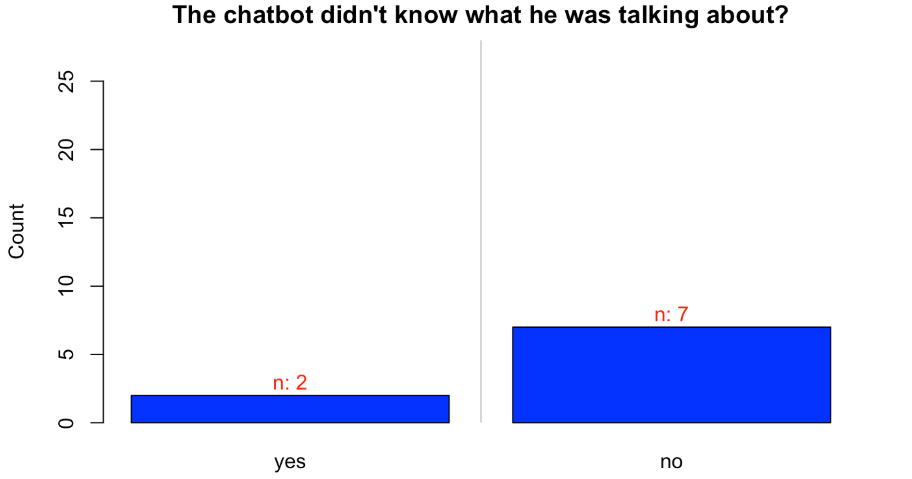
\includegraphics[width=\linewidth]{../LaTeX/Figures/Comparative/DQ3P.png}
	\caption{Bar chart of the responses for Proximus about the dysfunctional question for attribute 3, question 1.}\label{fig:DQ3P}
	\endminipage\hfill
	\minipage{0.32\textwidth}
	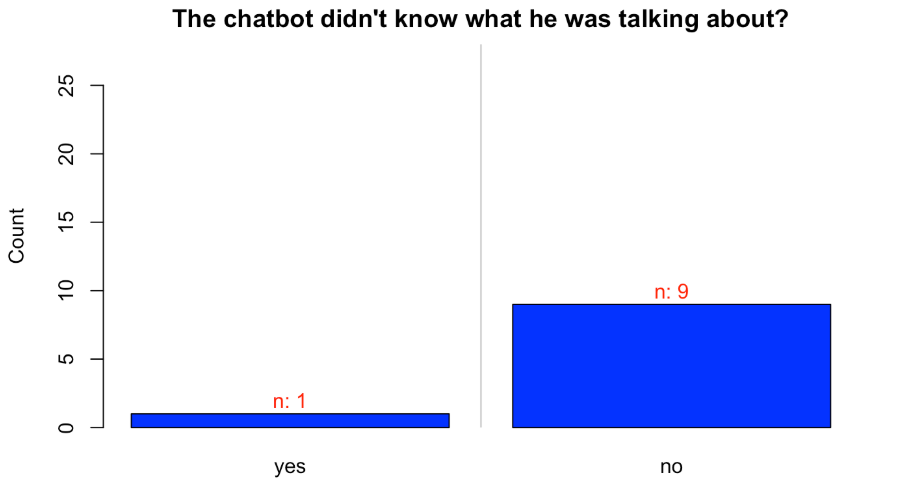
\includegraphics[width=\linewidth]{../LaTeX/Figures/Comparative/DQ3O.png}
	\caption{Bar chart of the responses for the others about the dysfunctional question for attribute 3, question 1.}\label{fig:DQ3O}
	\endminipage\hfill
\end{figure}
\break
The second question asks if the chatbot asked relevant questions to gather extra information about your problem. This question measures if the chatbot can gather more information if the given context isn't clear enough. Telenet and the others were mostly positive, Proximus has a 50-50 split.\\
\begin{figure}[!htb]
	\minipage{0.32\textwidth}
	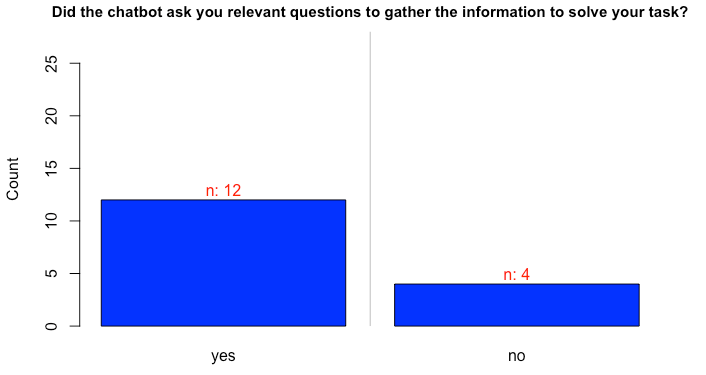
\includegraphics[width=\linewidth]{../LaTeX/Figures/Comparative/Q3Tb.png}
	\caption{Bar chart of the responses for Telenet about the functional question for attribute 3, question 2.}\label{fig:Q3Tb}
	\endminipage\hfill
	\minipage{0.32\textwidth}
	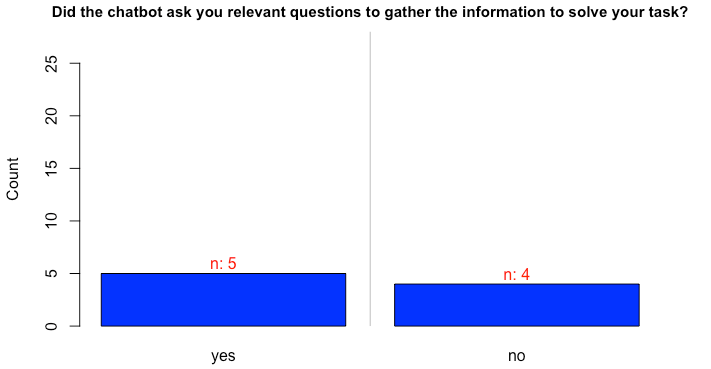
\includegraphics[width=\linewidth]{../LaTeX/Figures/Comparative/Q3Pb.png}
	\caption{Bar chart of the responses for Proximus about the functional question for attribute 3, question 2.}\label{fig:Q3Pb}
	\endminipage\hfill
	\minipage{0.32\textwidth}
	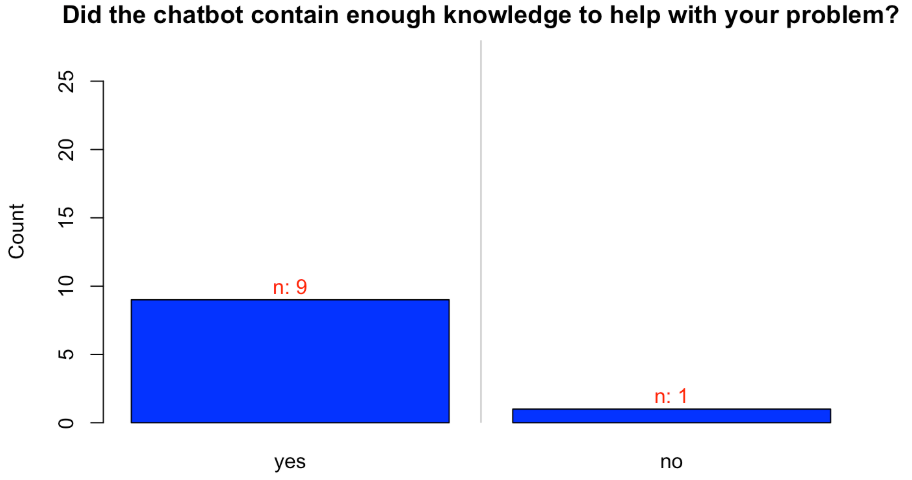
\includegraphics[width=\linewidth]{../LaTeX/Figures/Comparative/Q3O.png}
	\caption{Bar chart of the responses for the others about the functional question for attribute 3, question 2.}\label{fig:Q3Ob}
	\endminipage\hfill
\end{figure}
When looking at the reverse, Telenet seemed to not ask the right questions whereas Proximus and the others were about evenly split.\\
\begin{figure}[!htb]
	\minipage{0.32\textwidth}
	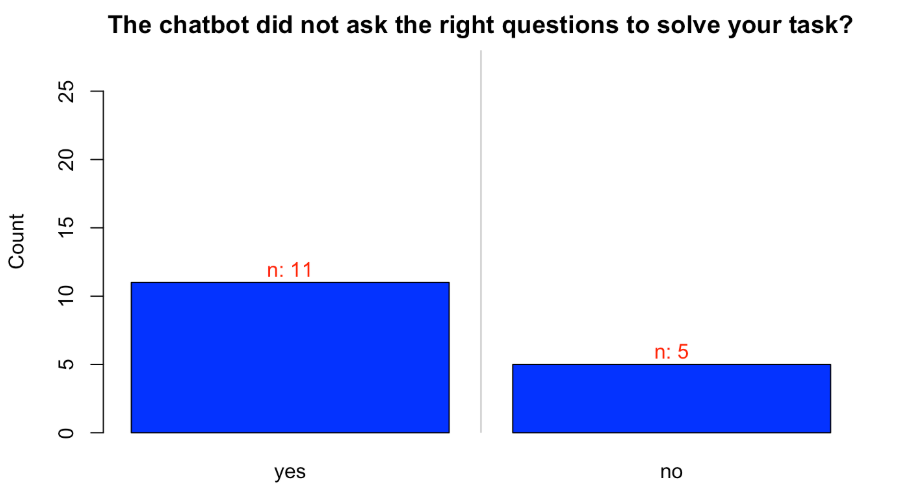
\includegraphics[width=\linewidth]{../LaTeX/Figures/Comparative/DQ3Tb.png}
	\caption{Bar chart of the responses for Telenet about the dysfunctional question for attribute 3, question 2.}\label{fig:DQ3Tb}
	\endminipage\hfill
	\minipage{0.32\textwidth}
	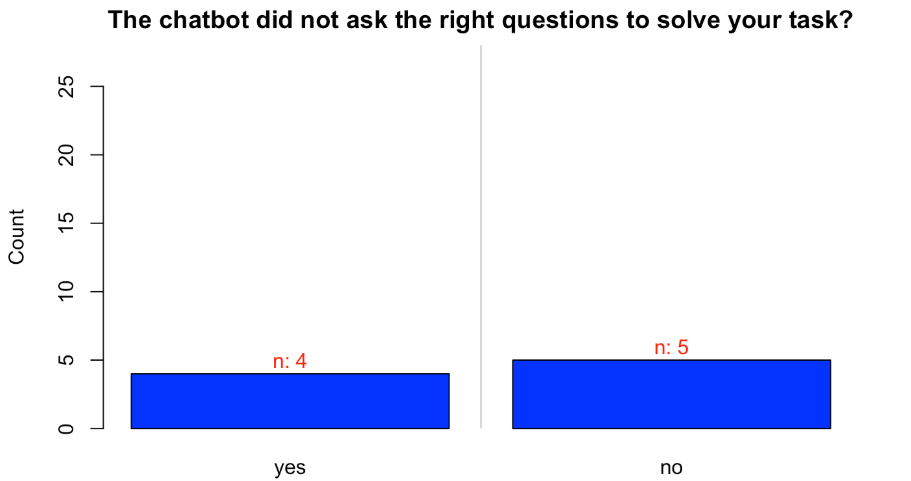
\includegraphics[width=\linewidth]{../LaTeX/Figures/Comparative/DQ3Pb.png}
	\caption{Bar chart of the responses for Proximus about the dysfunctional question for attribute 3, question 2.}\label{fig:DQ3Pb}
	\endminipage\hfill
	\minipage{0.32\textwidth}
	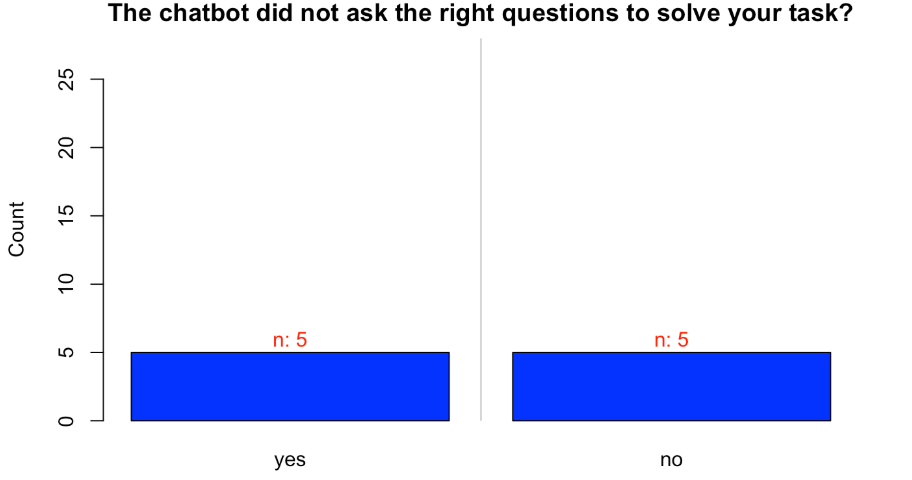
\includegraphics[width=\linewidth]{../LaTeX/Figures/Comparative/DQ3Ob.png}
	\caption{Bar chart of the responses for the others about the dysfunctional question for attribute 3, question 2.}\label{fig:DQ3Ob}
	\endminipage\hfill
\end{figure}
\break 
\ul{Attribute 4: Ease of use}\\
\break
\begin{figure}[!htb]
	\minipage{0.32\textwidth}
	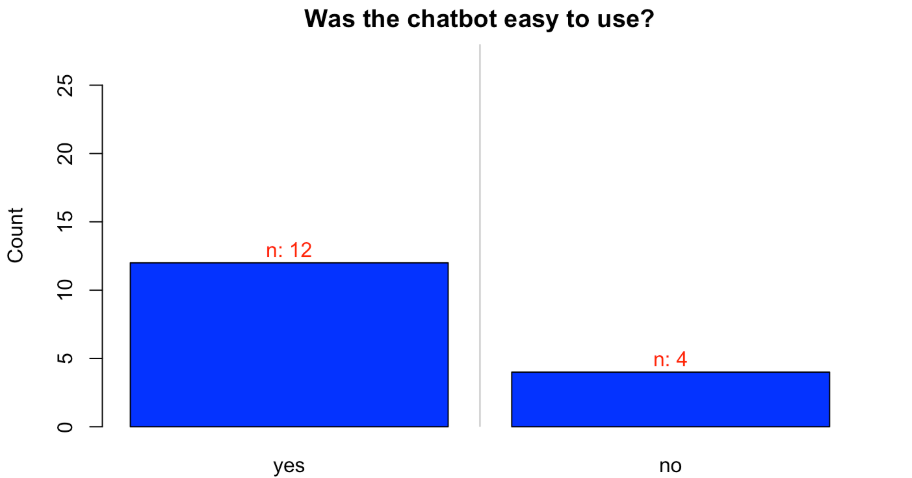
\includegraphics[width=\linewidth]{../LaTeX/Figures/Comparative/Q4T.png}
	\caption{Bar chart of the responses for Telenet about the functional question for attribute 4.}\label{fig:Q4T}
	\endminipage\hfill
	\minipage{0.32\textwidth}
	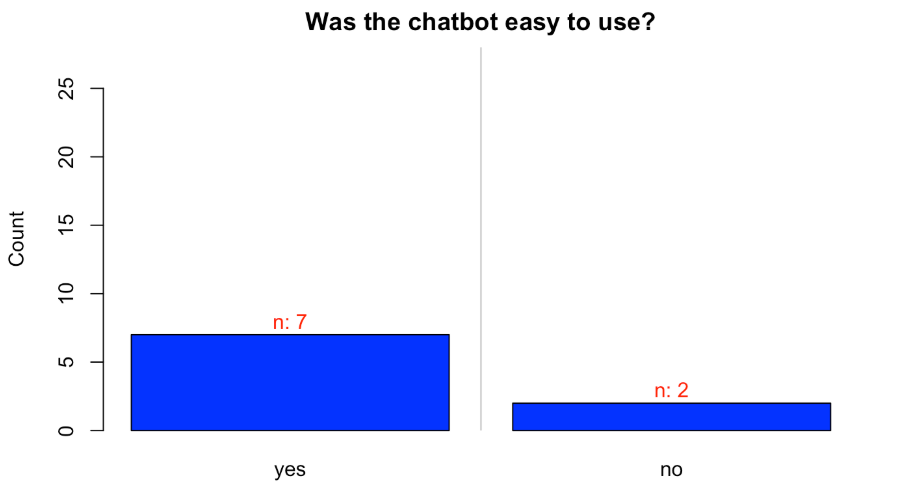
\includegraphics[width=\linewidth]{../LaTeX/Figures/Comparative/Q4P.png}
	\caption{Bar chart of the responses for Proximus about the functional question for attribute 4.}\label{fig:Q4P}
	\endminipage\hfill
	\minipage{0.32\textwidth}
	\includegraphics[width=\linewidth]{../LaTeX/Figures/Comparative/Q4O.png}
	\caption{Bar chart of the responses for the others about the functional question for attribute 4.}\label{fig:Q4O}
	\endminipage\hfill
\end{figure}
There weren't any complications when using the Telenet and Proximus chatbot or the chatbot provided by the others. Looking at the dysfunctional version of this question, the values confirm what's been seen for Telenet and the others but dispute the result for Proximus. There seem to be some problems when using the Proximus chatbot.\\
\begin{figure}[!htb]
	\minipage{0.32\textwidth}
	\includegraphics[width=\linewidth]{../LaTeX/Figures/Comparative/DQ4T.png}
	\caption{Bar chart of the responses for Telenet about the dysfunctional question for attribute 4.}\label{fig:DQ4T}
	\endminipage\hfill
	\minipage{0.32\textwidth}
	\includegraphics[width=\linewidth]{../LaTeX/Figures/Comparative/DQ4P.png}
	\caption{Bar chart of the responses for Proximus about the dysfunctional question for attribute 4.}\label{fig:DQ4P}
	\endminipage\hfill
	\minipage{0.32\textwidth}
	\includegraphics[width=\linewidth]{../LaTeX/Figures/Comparative/DQ4O.png}
	\caption{Bar chart of the responses for the others about the dysfunctional question for attribute 4.}\label{fig:DQ4O}
	\endminipage\hfill
\end{figure}
\break
\ul{Attribute 5: Enjoyable interaction}\\
\break
The 5\textsuperscript{th} and final attribute takes into consideration the interaction a user has with the chatbot. The first question asked if the chatbot was polite. The data shows that every group generally has a polite chatbot.\\
\begin{figure}[!htb]
	\minipage{0.32\textwidth}
	\includegraphics[width=\linewidth]{../LaTeX/Figures/Comparative/Q5T.png}
	\caption{Bar chart of the responses for Telenet about the functional question for attribute 5, question 1.}\label{fig:Q5T}
	\endminipage\hfill
	\minipage{0.32\textwidth}
	\includegraphics[width=\linewidth]{../LaTeX/Figures/Comparative/Q5P.png}
	\caption{Bar chart of the responses for Proximus about the functional question for attribute 5, question 1.}\label{fig:Q5P}
	\endminipage\hfill
	\minipage{0.32\textwidth}
	\includegraphics[width=\linewidth]{../LaTeX/Figures/Comparative/Q5O.png}
	\caption{Bar chart of the responses for the others about the functional question for attribute 5, question 1.}\label{fig:Q5O}
	\endminipage\hfill
\end{figure}
\break
When asked if the chatbot interacted in a respectful way, the answers for Telenet were mostly positive, Proximus is once again divided around the 50\% mark and the others scored 100\%.\\
\begin{figure}[!htb]
	\minipage{0.32\textwidth}
	\includegraphics[width=\linewidth]{../LaTeX/Figures/Comparative/DQ5T.png}
	\caption{Bar chart of the responses for Telenet about the dysfunctional question for attribute 5, question 1.}\label{fig:DQ5T}
	\endminipage\hfill
	\minipage{0.32\textwidth}
	\includegraphics[width=\linewidth]{../LaTeX/Figures/Comparative/DQ5P.png}
	\caption{Bar chart of the responses for Proximus about the dysfunctional question for attribute 5, question 1.}\label{fig:DQ5P}
	\endminipage\hfill
	\minipage{0.32\textwidth}
	\includegraphics[width=\linewidth]{../LaTeX/Figures/Comparative/DQ5O.png}
	\caption{Bar chart of the responses for the others about the dysfunctional question for attribute 5, question 1.}\label{fig:DQ5O}
	\endminipage\hfill
\end{figure}
\break
The second question askes if the user liked interacting with the chatbot. This time, Telenet is evenly split and both Proximus and the others are mostly positive.\\
\begin{figure}[!htb]
	\minipage{0.32\textwidth}
	\includegraphics[width=\linewidth]{../LaTeX/Figures/Comparative/Q5Tb.png}
	\caption{Bar chart of the responses for Telenet about the functional question for attribute 5, question 2.}\label{fig:Q5Tb}
	\endminipage\hfill
	\minipage{0.32\textwidth}
	\includegraphics[width=\linewidth]{../LaTeX/Figures/Comparative/Q5Pb.png}
	\caption{Bar chart of the responses for Proximus about the functional question for attribute 5, question 2.}\label{fig:Q5Pb}
	\endminipage\hfill
	\minipage{0.32\textwidth}
	\includegraphics[width=\linewidth]{../LaTeX/Figures/Comparative/Q5Ob.png}
	\caption{Bar chart of the responses for the others about the functional question for attribute 5, question 2.}\label{fig:Q5Ob}
	\endminipage\hfill
\end{figure}
When asked the reverse, both Telenet and the others are divided evenly. Proximus has more negative than positive responses meaning for the users of Proximus, it wasn't a task to interact with their chatbot.\\
\begin{figure}[!htb]
	\minipage{0.32\textwidth}
	\includegraphics[width=\linewidth]{../LaTeX/Figures/Comparative/DQ5Tb.png}
	\caption{Bar chart of the responses for Telenet about the dysfunctional question for attribute 5, question 2.}\label{fig:DQ5Tb}
	\endminipage\hfill
	\minipage{0.32\textwidth}
	\includegraphics[width=\linewidth]{../LaTeX/Figures/Comparative/DQ5Pb.png}
	\caption{Bar chart of the responses for Proximus about the dysfunctional question for attribute 5, question 2.}\label{fig:DQ5Pb}
	\endminipage\hfill
	\minipage{0.32\textwidth}
	\includegraphics[width=\linewidth]{../LaTeX/Figures/Comparative/DQ5Ob.png}
	\caption{Bar chart of the responses for the others about the dysfunctional question for attribute 5, question 2.}\label{fig:DQ5Ob}
	\endminipage\hfill
\end{figure}
\subsection{Importance Study - Kano}
\subsubsection{Discrete analysis}
To start with the KANO analysis, there first had to be made a clear mapping between the functional and dysfunctional question and which label of KANO would be assigned to the outcome of this mapping. The mapping can be found in Figure \ref{fig:kanoOverview}.
\begin{figure}[htb!]
	\centering
	\includegraphics[width=\linewidth]{../LaTeX/Figures/Kano/KANOOverview.png}
	\caption{The mapping between the functional and dysfunctional question and the KANO label associated.}
	\label{fig:kanoOverview}
\end{figure}
\break
\break
Afterwards, for each scenario (see 3\textsuperscript{rd} part of the survey description) as well as the general questions of the survey, the answers were counted and added per label. The highest label was assigned. If there was an overlap between two or more labels, the label with the most impact was chosen. The order of impact is:
\begin{enumerate}
	\item Attractive
	\item Performance
	\item Must-be
	\item Indifference
	\item Reverse
\end{enumerate}
An overview  of the label assigned to each entry can be found in Figure \ref{fig:kanoTable}. S1, S2 and S3 refer to the 3 different scenarios within which the questions were asked.
\begin{figure}[!htb]
	\centering
	\includegraphics[width=\linewidth]{../LaTeX/Figures/Kano/KanoTable.png}
	\caption{Each entry with it's assigned KANO label.}
	\label{fig:kanoTable}
\end{figure}
\subsubsection{Continuous analysis}
Now, each entry has a label assigned to it and for every entry, the different categories are counted. Based on this, both the satisfaction as well as the dissatisfaction coefficient can be calculated. The calculations can be seen in Figure \ref{fig:satisfactionCoef} and Figure \ref{fig:dissatisfactionCoef}.
\begin{figure}[!htb]
	\centering
	\includegraphics{../LaTeX/Figures/Kano/SatisfactionCoef.png}
	\caption{The satisfaction coefficient.}
	\label{fig:satisfactionCoef}
\end{figure}
\begin{figure}[!htb]
	\centering
	\includegraphics{../LaTeX/Figures/Kano/DissatisfactionCoef.png}
	\caption{The dissatisfaction coefficient.}
	\label{fig:dissatisfactionCoef}
\end{figure}
\break
After calculating both these scores for each entry, they were plotted in  a scatter plot, dividing them up into one of the four main categories of KANO. The categorisation can be found in Figure \ref{fig:satisfactionPlot}
\begin{figure}[!htb]
	\centering
	\includegraphics[width=\linewidth]{../LaTeX/Figures/Kano/SatisfactionPlot.png}
	\caption{The satisfaction/dissatisfaction plot.}
	\label{fig:satisfactionPlot}
\end{figure}

\begin{longtable}{|c|l|}
	\hline
	\textbf{Item} & \multicolumn{1}{c|}{\textbf{Attribute}}         \\ \hline
	\endfirsthead
	\endhead
	\textbf{1}    & S1: Execute requested tasks                     \\ \hline
	\textbf{2}    & S1: Number of services available in the chatbot \\ \hline
	\textbf{3}    & S1: Contains breadth of knowledge               \\ \hline
	\textbf{4}    & S2: Execute requested tasks                     \\ \hline
	\textbf{5}    & S2: Number of services available in the chatbot \\ \hline
	\textbf{6}    & S2: Contains breadth of knowledge               \\ \hline
	\textbf{7}    & S3: Execute requested tasks                     \\ \hline
	\textbf{8}    & S3: Number of services available in the chatbot \\ \hline
	\textbf{9}    & S3: Contains breadth of knowledge               \\ \hline
	\textbf{10}   & Available at all times                          \\ \hline
	\textbf{11}   & Ease of use                                     \\ \hline
	\textbf{12}   & Create an enjoyable interaction                 \\ \hline
	\caption{An Overview of the plotted entries in the satisfaction/dissatisfaction plot.}
	\label{tab:kanoSatisfactionDissatisfactionTable}
\end{longtable}

\section{Discussion}
\subsubsection{RQ1: Are current customer service chatbots effective in helping people and
	solving their problems?}
\ul{H1: Current customer service chatbots execute requested tasks correctly.}\\
At this point, there seems to be a split customer base about the delivered service by the chatbot. Some are happy with the execution of their task where others weren't. They also indicate that the chatbot needs help from an agent but this seemed to match their expectations. In the end, most could solve their problem with the help of the chatbot.\\
\break
\ul{H2: Current customer service chatbots can deliver the same services as a human
	agent.}\\
The data clearly shows that people don't think chatbots can deliver the same services as a human agent to the same quality.\\
\break
\ul{H3: Current customer service chatbots contain enough knowledge to provide good
	assistance.}\\
Here again, seems to be a big split between the customers. Depending on the provider, around 50\% think the chatbot is knowledgeable enough to help with their problem. When the chatbot didn't have enough context to solve a question, depending on the situation, around 50\% think the chatbot did not ask the right questions to gather the needed information.\\
\break
\textbf{RQ1:} The opinions are divided. In some cases they are effective, in others they aren't but they perform up to expectations from the customer.\\
\subsubsection{RQ2: Are current customer service chatbots easy to use and accessible?}
\ul{H4: Current customer service chatbots are easy to use.}\\
In general, there doesn't seem to be a problem when using the chatbot.\\
\break
\ul{H5: Current customer service chatbots are available at all times (24/7).}\\
Each provider provides a chatbot that is available 24/7.\\
\break
\textbf{RQ2:} Yes, chatbots are easy to use and accessible.\\
\subsubsection{RQ3: Do current customer service chatbots create a pleasant customer experience?}
\ul{H6: Current customer service chatbots create an enjoyable interaction.}\\
Chatbots are generally perceived to be polite to interact with and most didn't mind interacting with a chatbot.\\
\break
\textbf{RQ3:} It's not yet perceived as enjoyable but it isn't a task either.\\

\subsection{Quality attributes for telecom chatbots}
\ul{Difference between the scenarios}\\
Looking at the labels assigned to each category in each scenario, it is clear that there isn't much difference in importance between the different scenarios. Looking at Figure \ref{fig:satisfactionPlot}, the same attributes for different scenarios are quite close together as well.\\
\break
\ul{General attributes}\\
Ease of use turns out to be a must-be. Compared to the comparative study, this matches the found conclusion and corresponding responses.\\
Availability is a performance attribute. If not/less present, the valued perception of the chatbot would diminish.\\
Customers are indifferent about the experience created by the chatbot. Comparing this to the comparative study, this matches the found answer to RQ3.

\subsection{The future vision of telecom chatbots}
The various interviews revealed how customer service chatbots will evolve within the telecom sector and what the most important improvement points are. First and foremost, telecom providers are trying to further optimise their services by applying further data analysis and fine-tuning algorithms. They are also looking at sentiment analysis to map out the mood of the customer in order to enable the chatbot to anticipate this. They are also looking at making the chatbots more compatible in terms of language by means of APIs. As discussed earlier, chatbots are offered on different platforms, and one of the focal points that was discussed several times was to harmonise these different platforms so that the chatbot is aware of when it is communicating via another platform. In the long term, it can be expected that voice bots will also become more prevalent with possible integrations to smart speakers such as Google home and Alexa.


